%! Author = giaco
%! Date = 16/05/2024

\chapter{Experiments \& Results}
\label{ch:experiments_and_results}
In this chapter we are going to provide information about the experiments that we conducted to test our agents along with the results obtained.
We start by describing the experimental setup in Sec. \ref{sec:exp_setup}, talking about the libraries and tools used, the data collected, and the training process.
Then, in Sec. \ref{subsec:init_exp}, we present the initial experiments that we conducted to find the best performing extractors for each game.
%TODO EXTEND

\section{Experimental Setup}\label{sec:exp_setup}
To simulate and interact with the Atari environments~\citep{bellemare2013atari} we leveraged the API provided by Gymnasium~\citep{towers_gymnasium_2023}, which has extensive support for Atari games and has been widely used in the RL community.
The training performance was tracked using \texttt{Weights and Biases}~\citep{wandb}, that allows to monitor the agents and store the results in a cloud-based platform.
In particular, we utilized the interface provided by SB3, which allowed us to decompose the agents' network into a \textit{Feature Extractor} and \textit{Fully-Connected Network}, as also highlighted in Figure~\ref{fig:main_architecture}.
We used the \textit{Feature Extractor} to implement the different combination modules providing as output the composed latent representation.
The \textit{Fully-Connected Network} is kept as simple as possible, this is because most of the information should be provided by the FMs' representations.
It receives as input the FMs' combined linear encoding and subsequently maps it to actions (or values).

In the execution of all experiments, we maintained the hyperparameters provided by \citet{rl-zoo3} for different RL algorithms.
We did not conduct any hyperparameter search this time, this to avoid adding complexity to the experiments and growing the time.
Instead, we only modify the model architecture.
All the values are reported in Appendix \ref{sec:app-exp-setup}.
The experiments were conducted on a machine equipped with 4 Intel Xeon Gold 6140M CPUs for a total of 144 threads, 4 Nvidia Tesla V100 GPUs with 16GB of memory, and 1.2TB of RAM.
The experiments were conducted on a single GPU, eventually running multiple experiments in parallel.


\subsection{FMs Data and Training}\label{subsec:fms-data-and-training}
For the main experiments of our approach, we use three different models which provides us four different pre-trained networks: \texttt{Video Object Segmentation} (VOS)~\citep{goel2018unsupervised}, \texttt{State Representation} (SR)~\citep{anand2019unsupervised}, and finally \texttt{Object Keypoints}~\citep{kulkarni2019unsupervised} which provides us the encoder (OKE) and the keypoint network (OKK).
These models constitute the set of basic skills that the agent is equipped with.
We believe that these models provide a good starting point for the agent to learn the environment, and they are informative enough to provide a good representation of the state.
SR gives a general representation of the state in a compact form, VOS tracks moving objects in the frame, and OKK provides the agent with the position of the objects.

Additionally, for attention-based combination modules, we train a deep autoencoder - inspired by Nature CNN~\citep{mnih2015human} - to encode the current state and leverage its representation to compute the context.
The architecture of Nature CNN has been slightly modified as it appears in Tab. \ref{tab:nature_cnn} to
match the dimensions of other FMs' representations.


\begin{table}[htbp]
     \begin{center}
         \begin{tabular}{lllll}
             \multicolumn{1}{l}{\bf Layer}  & \multicolumn{1}{l}{\makecell{\bf In.\\\bf Channels}}  & \multicolumn{1}{l}{\makecell{\bf Out.\\\bf Channels}}  & \multicolumn{1}{l}{\makecell{\bf Kernel\\\bf size}}  & \multicolumn{1}{l}{\bf Stride}
             \\ \hline \\
             1st CNN Layer   &  1  & 32 & 8 & 4 \\
             2nd CNN Layer   &  32  & 64 & 3 & 1 \\
             3rd CNN Layer   &  64  & 64 & 3 & 1 \\
         \end{tabular}
     \end{center}
     \caption{This table shows the encoder architecture of the Deep Autoencoder. It takes as input only the last frame in grayscale. The stride on the second convolutional layer was decreased from 2 to 1 with respect to Nature CNN. Each convolutional layer is followed by a ReLU activation function. The decoder part is specular.}
     \label{tab:nature_cnn}
 \end{table}




To train the different FMs we first create a specific dataset for each game.
For each environment, we collected \texttt{1M} frames via agents interacting with the environment.
The agents act randomly in this case, and the frames are collected without any reward.
This is done to ensure that the data is not biased towards a specific policy.
The dataset contains grayscaled game frames with size 84x84 pixels.
During the training process of the models, data is randomly sampled to avoid any correlation between elements due to the collection phase.
We implement and train the models for all the games using the default architecture and hyperparameters, the values and additional details are reported in Appendix~\ref{sec:app-models}.
While training the agent, pre-trained models' weights are frozen and no longer updated.

These FMs are small models which can be easily changed to more complex models without affecting the structure of our work if needed.
As previously mentioned, the main objective of this work is the combination of different representations.


\section{Initial Experiments}\label{sec:init_exp}
As showed in Section~\ref{sec:environments}, we chose three different Atari games as benchmark for our work, namely \textit{Pong, Breakout, and Ms. Pacman,}
A first choice of the games was dictated by the availability of the RAM annotations provided in~\cite{anand2019unsupervised}.
Then to avoid adding complexity and growing the time for experiments we restricted to test only the games already cited.
We believe that this choice of games provides a fair compromise between simple games like Pong and much more complex games like Pacman.
For each environment, we selected the \textit{NoFrameskip-v4} version of the game.


After training each FMs, we run a first round of experiments for the three games to find the three best performing combination modules that will be used for our empirical analysis along with our proposed method.
Agents are trained for \texttt{10M} steps using the parameters provided by \texttt{rl-zoo}, and we use as RL algorithm PPO~\citep{schulman2017proximal}.
The \texttt{Fully-Connected Network} is set to a single layer of 256 units both for policy network and value function network.
Throughout the learning process, agents are repeatedly evaluated for 100 episodes.


As shown in Table~\ref{tab:emb_siz_modules}, we explore a variety of configurations for each module, ensuring a comprehensive assessment of their performance.
During the training phase of these first experiments, we applied early stopping for agents that showed no improvement over five consecutive evaluations.
This strategy allowed us to promptly identify the best-performing configurations and to save computational resources as these experiments are computationally expensive.


\begin{table}[ht]
    \begin{center}
        \begin{tabular}{ll}
            \multicolumn{1}{l}{\bf Feature Extractor}  &\multicolumn{1}{l}{\bf Embedding Size}
            \\ \hline \\
            LIN              &  - \\
            FIX        & 256, 512, 1024 \\
            CNN       & 1, 2, 3\\
            MIX                             & - \\
            RES           & 512, 1024, 2048 \\
            DPA             & 256, 512, 1024 \\
            WSA         & 256, 512, 1024 \\

        \end{tabular}
    \end{center}
    \caption{The table shows all the extractors' configurations tested in the initial phase of experiments. For FIX, DPA, and WSA the values indicate the fixed dimensions of embeddings and context, for RES the size of the reservoir and for CNN the number of convolutional layers.}
    \label{tab:emb_siz_modules}
\end{table}

In Appendix~\ref{sec:app-com-mod} we report all the learning curves in this experimental phase.

Here instead we show our first results providing the best performing modules for each game, the chosen embedding size is detailed between parentheses:
\begin{itemize}
    \item \texttt{Pong}: WSA (1024), RES (1024), CNN (2)
    \item \texttt{Ms.Pacman}: WSA (256), RES (1024), CNN (2)
    \item \texttt{Breakout}: WSA (256), FIX (512), CNN (3)
\end{itemize}

\section{Top 3 Performer}\label{sec:top-3-performer}
In the subsequent phase, the research progressed with a refined focus.
We used the same methodology and setup as the initial experiments for our empirical evaluation, but we restricted the tests only to the best performing modules for each game.
This time we avoid using early stopping, and we let the agents train for the full \texttt{10M} steps.
For each game, for each agent, we executed multiple instances of the experiment using different seeds for a total of \texttt{4} runs per agent per game.
The training results are averaged over the different seeds, and we also considered a Running Average of the cumulative reward to smooth the learning curves.
We also included the PPO agent as a reference, for a total of \texttt{4} agents per game.
Figure~\ref{fig:trainresults} shows the average learning curves of agents during training - the shaded area depicts the standard deviation.



\begin{figure}[ht]
    \centering
    \begin{subfigure}[b]{0.32\textwidth}
        \centering
        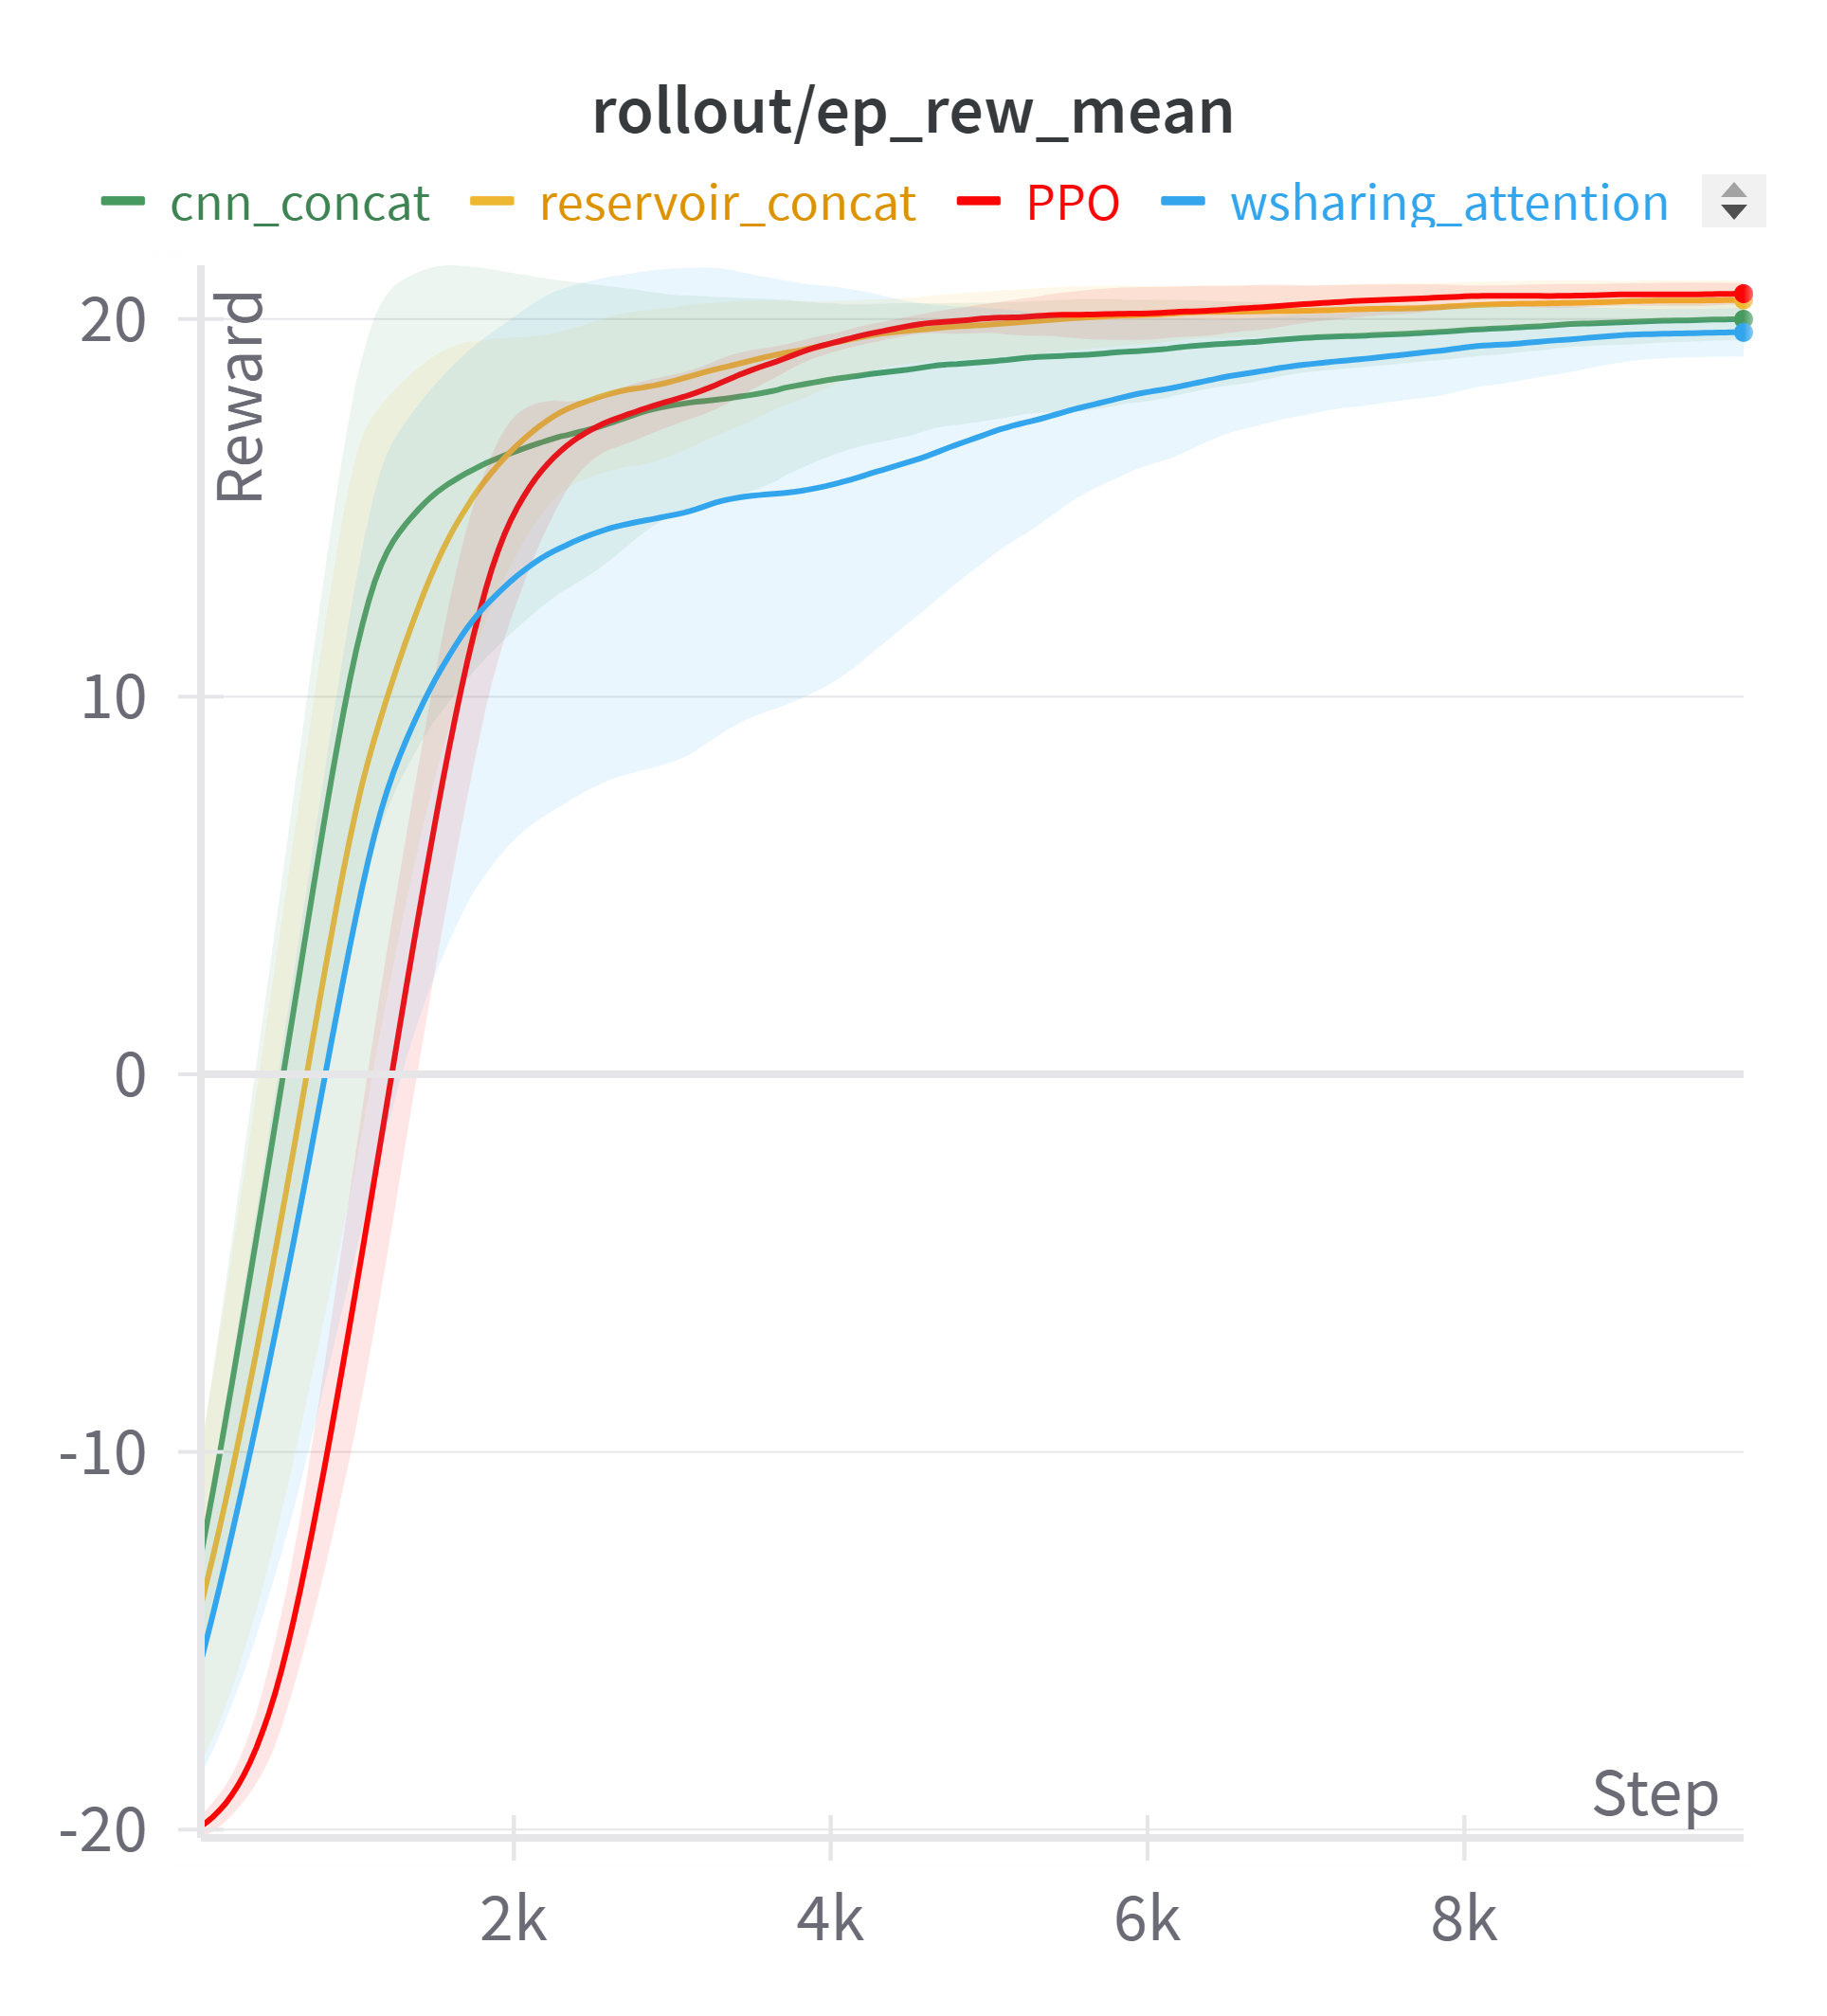
\includegraphics[width=\textwidth]{images/pong_train}
        \caption{\texttt{Pong}}
        \label{fig:pongtraining}
    \end{subfigure}
    \hfill
    \begin{subfigure}[b]{0.32\textwidth}
        \centering
        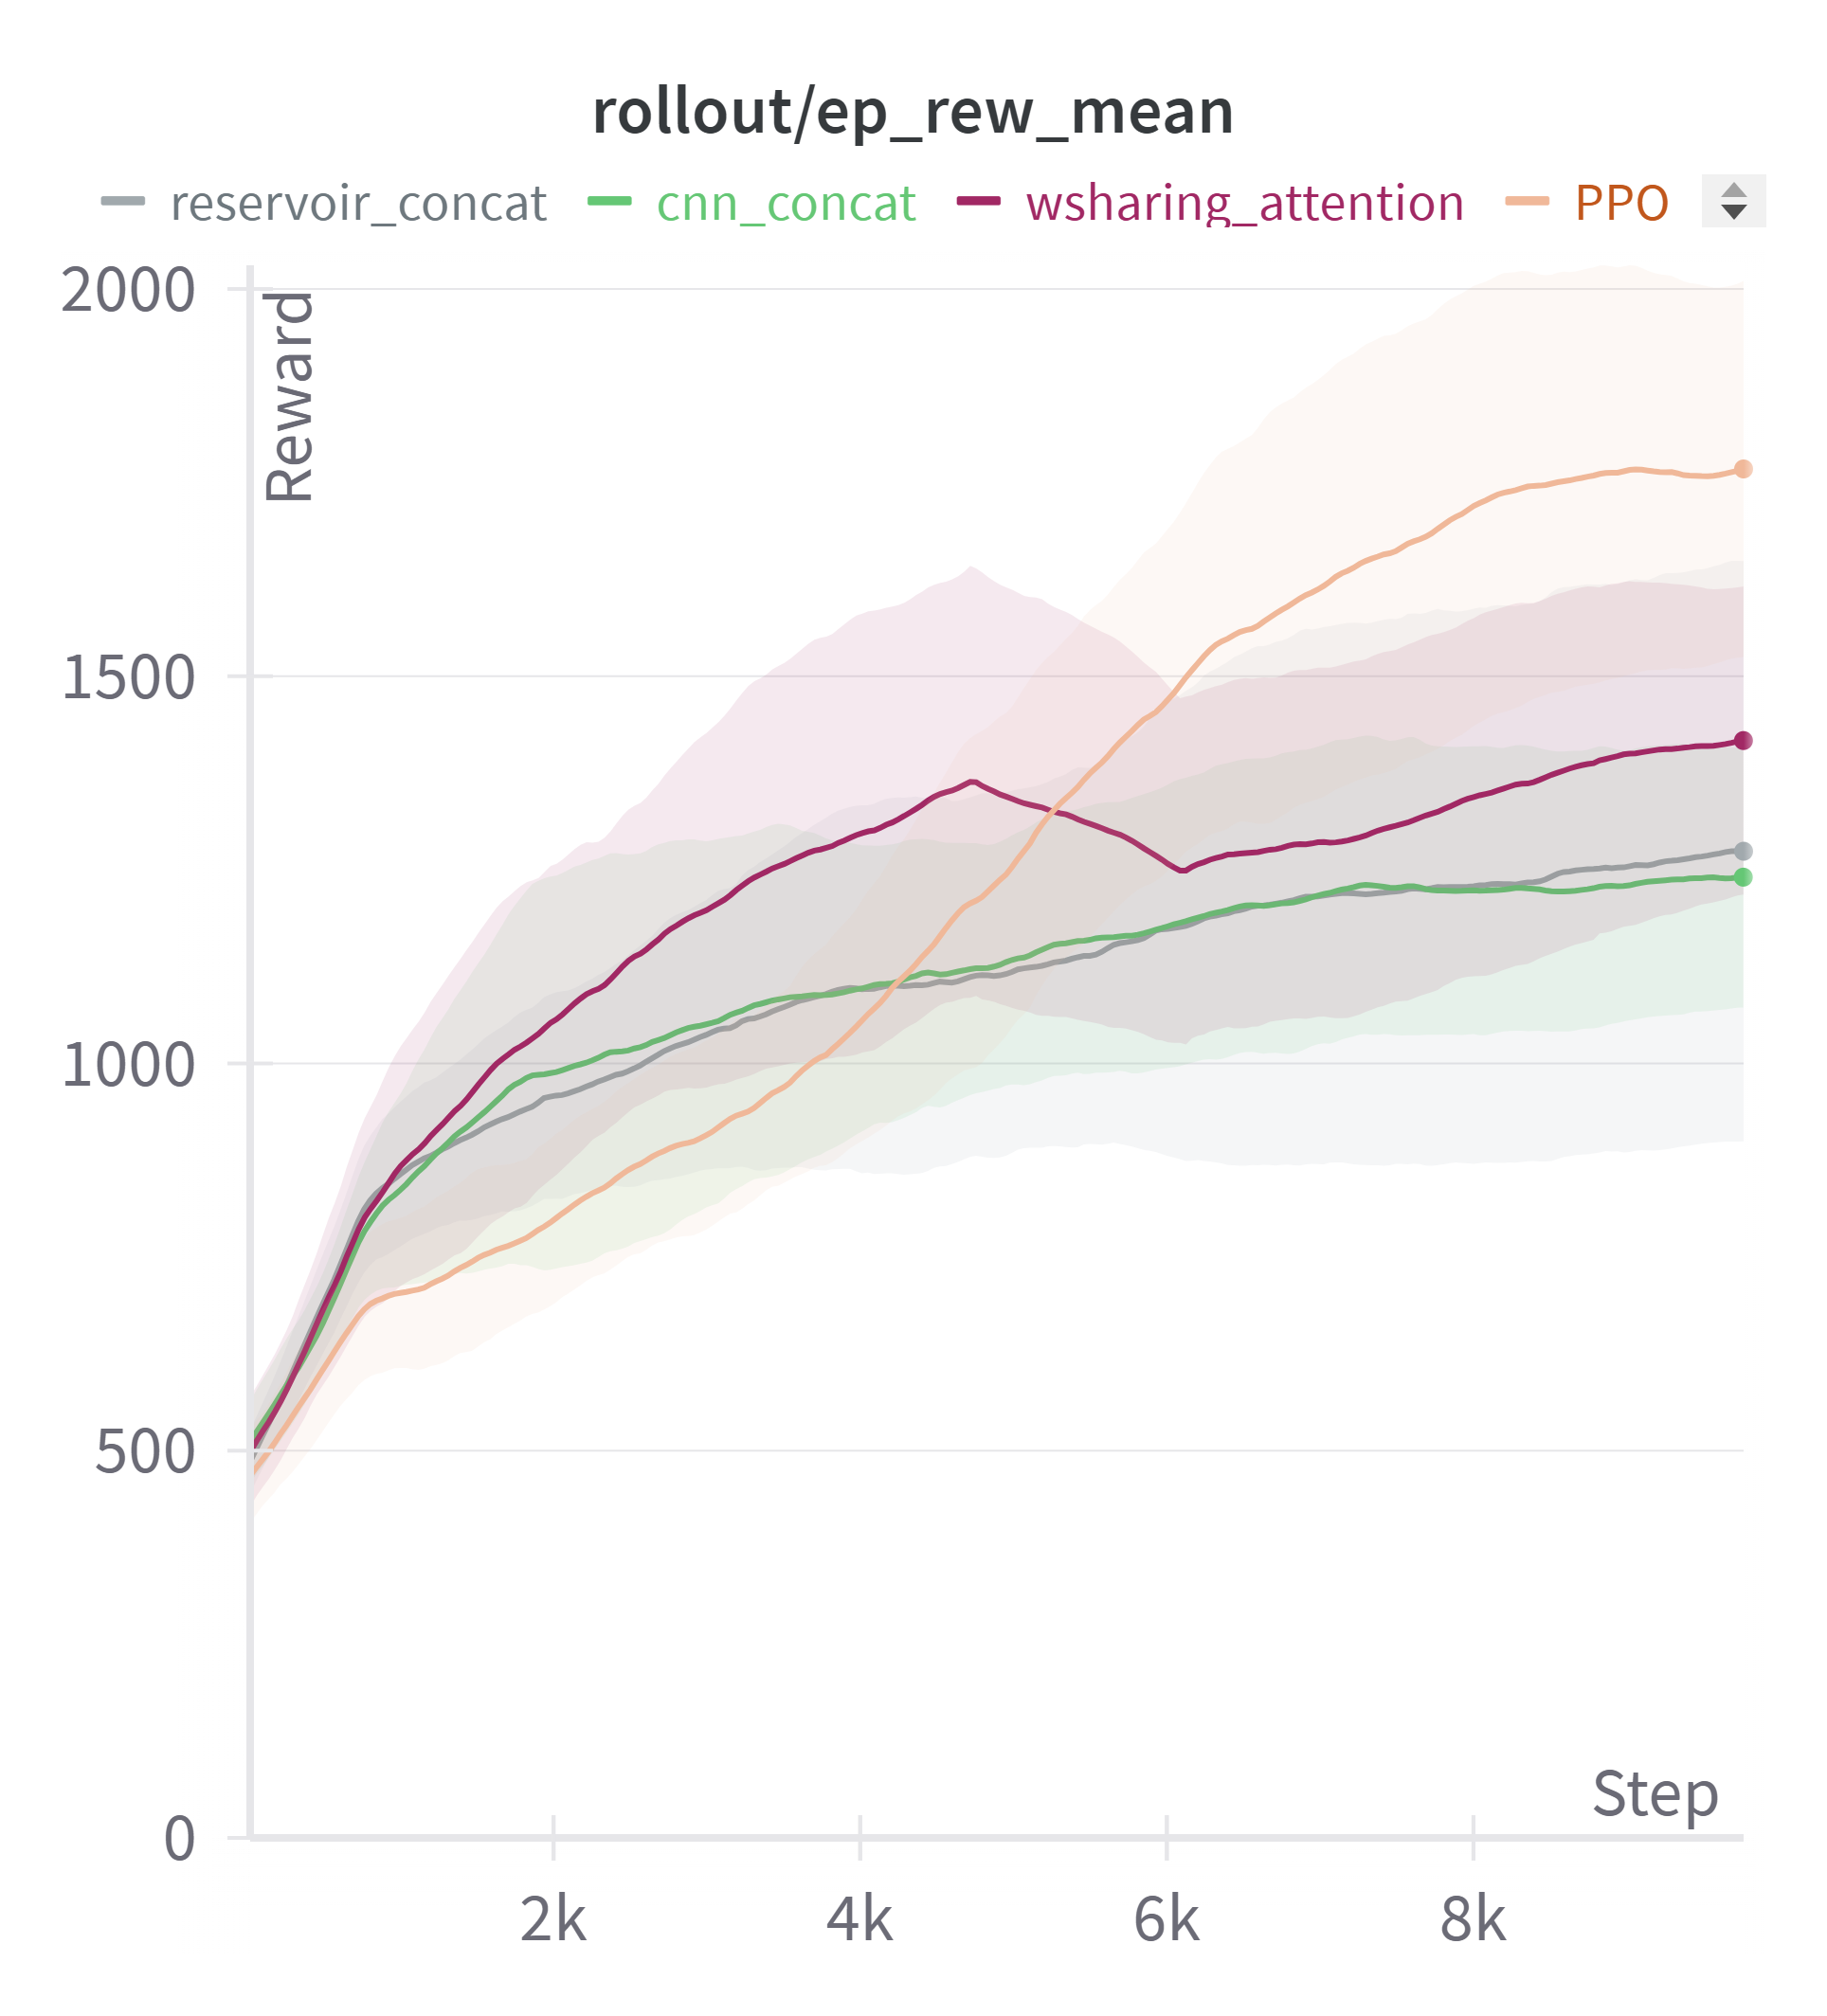
\includegraphics[width=\textwidth]{images/mspacman_train}
        \caption{\texttt{Ms.Pacman}}
        \label{fig:mspacmantrain}
    \end{subfigure}
    \hfill
    \begin{subfigure}[b]{0.32\textwidth}
        \centering
        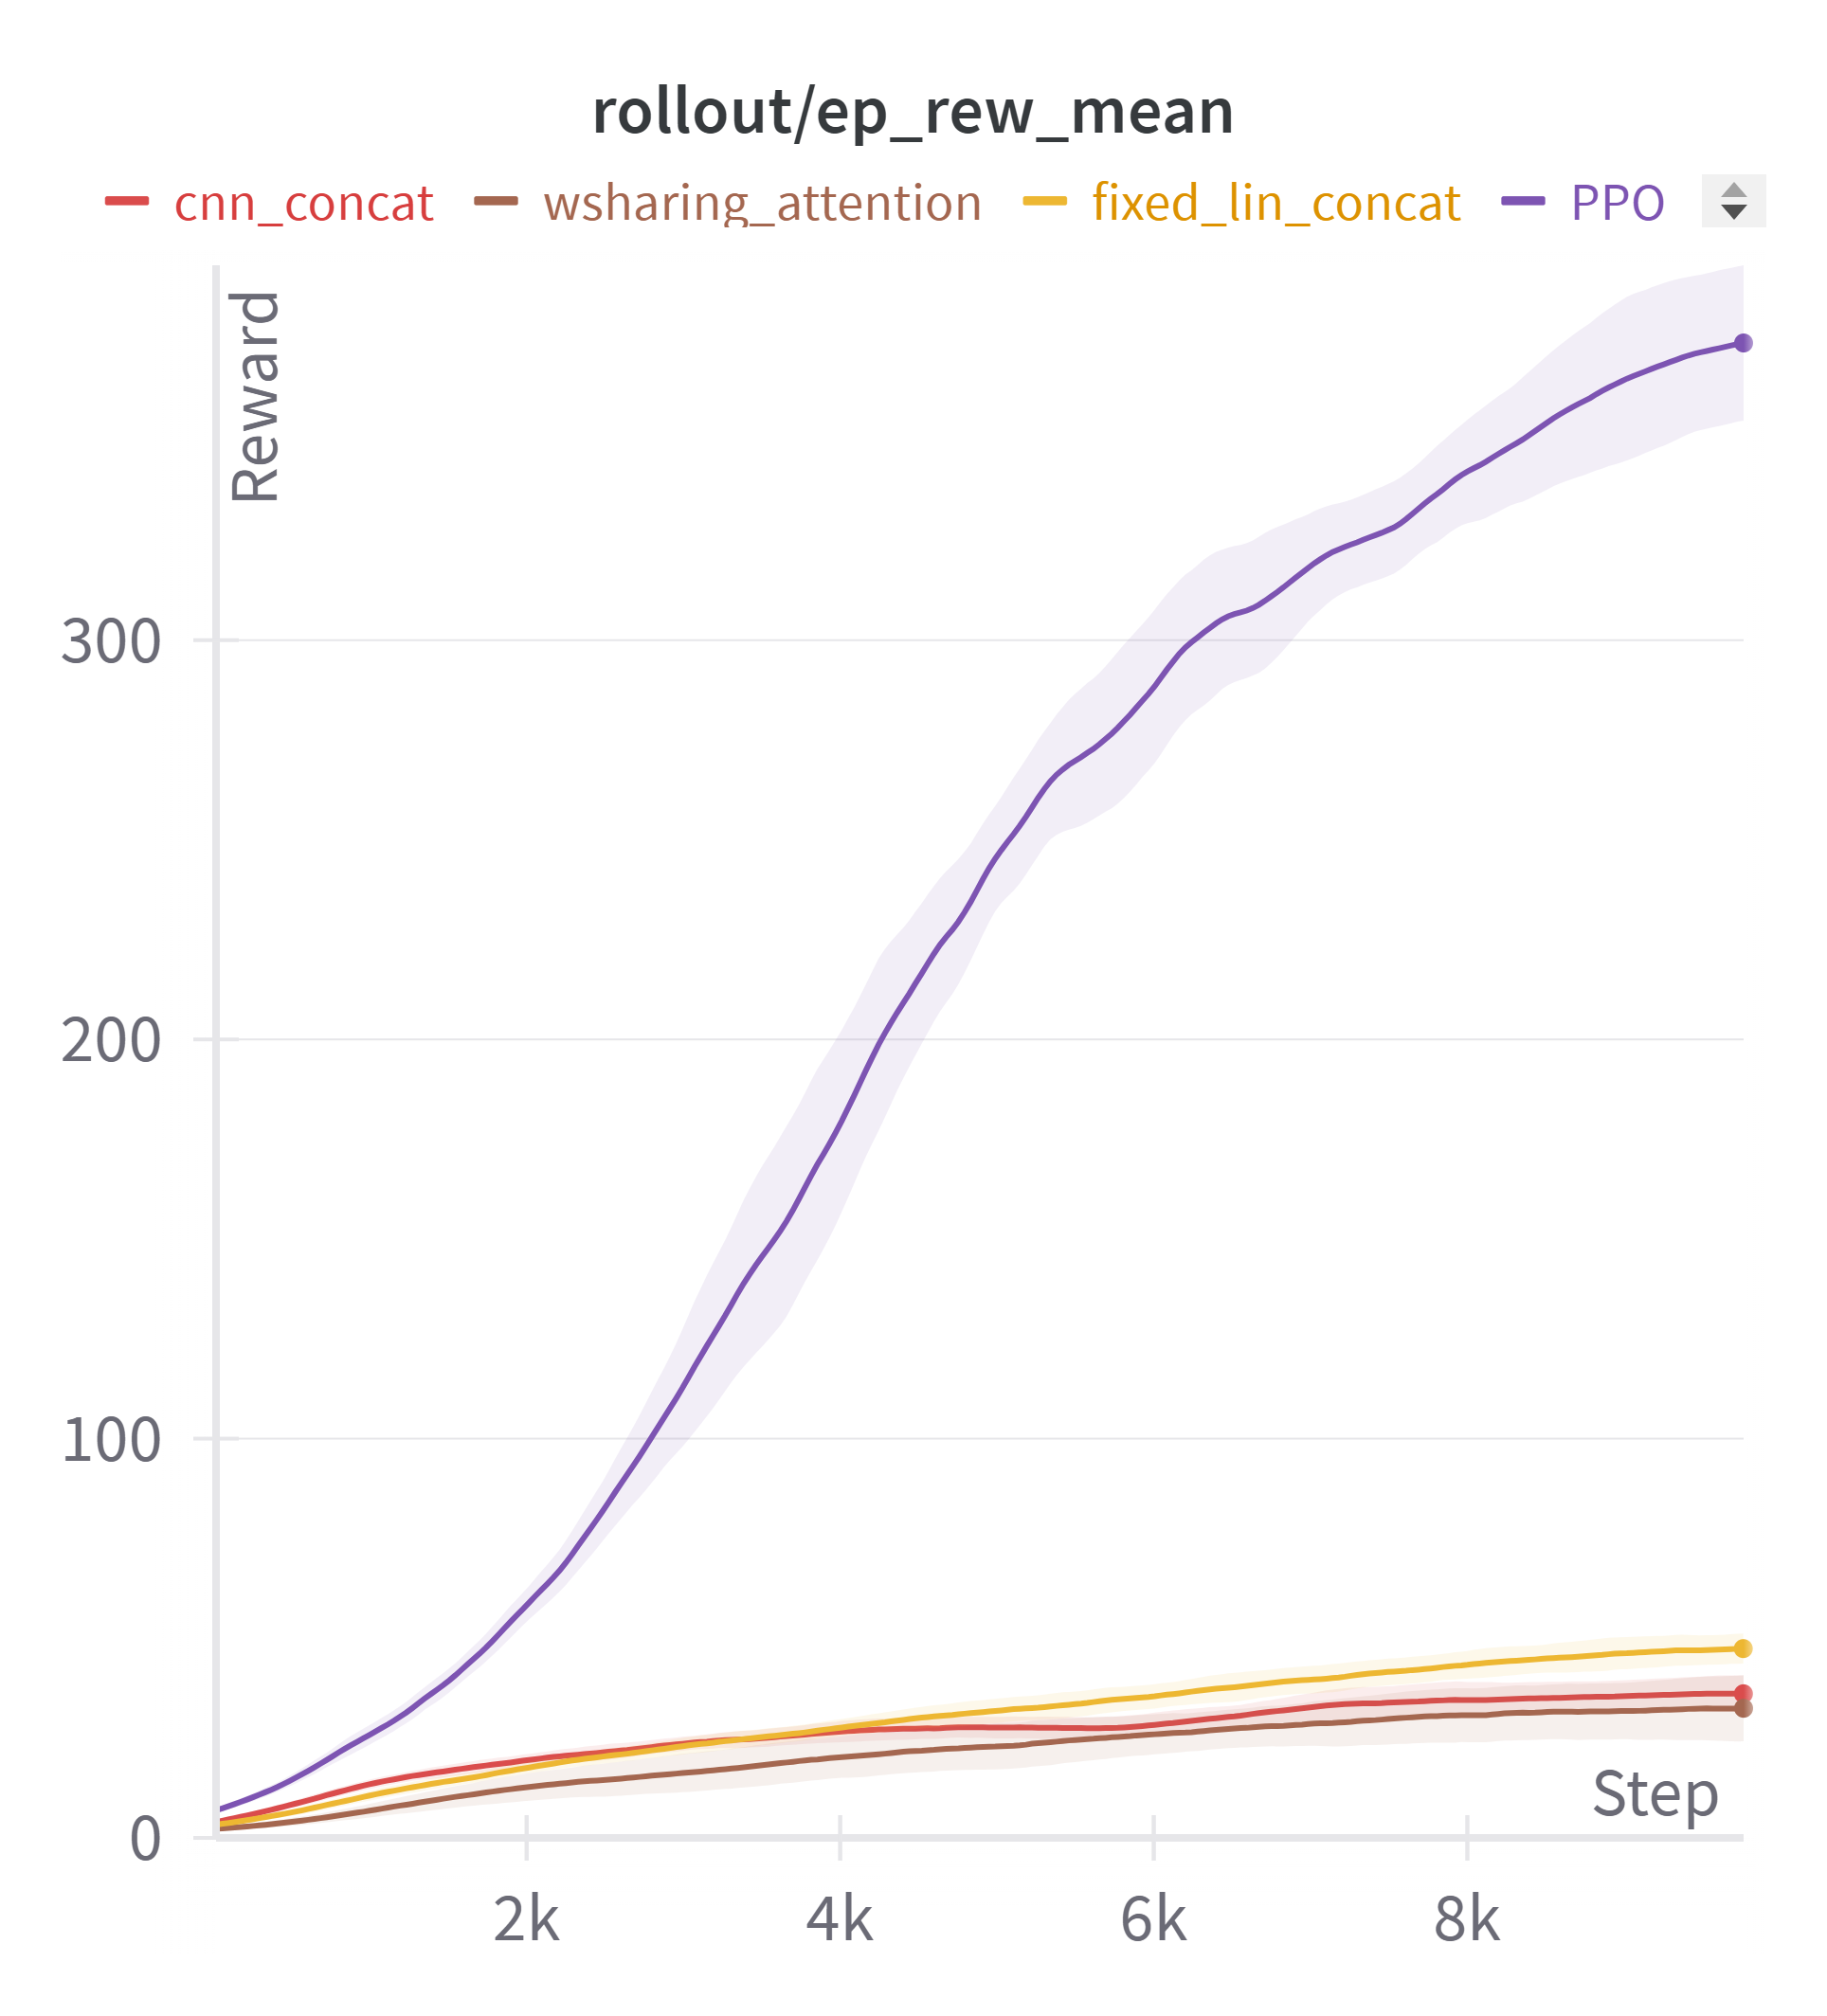
\includegraphics[width=\textwidth]{images/breakout_train}
        \caption{\texttt{Breakout}}
        \label{fig:breakouttrain}
    \end{subfigure}
    \caption{Cumulative reward during \texttt{training} of different agents, including WSA, PPO, and other combination modules, on three different Atari games. Each subfigure shows the mean score, with shaded areas indicating the standard deviations, across multiple agents.}
    \label{fig:trainresults}
\end{figure}


To evaluate our agents, we selected for each agent the model that performed best during training, and we tested it across \texttt{5 random seeds} for \texttt{50 episodes}.
The seeds specifically are: 47695, 32558, 94088, 71782 and 66638.
Table~\ref{tab:results} reports the averaged results during evaluation of the best agent during training.

\begin{table}[ht]
\centering
    \begin{tabular}[b]{lll}
                \multicolumn{1}{l}{Environment}  &\multicolumn{1}{l}{\bf Agent} &\multicolumn{1}{l}{\bf Reward} \\
                \hline \\
                \multirow{4}{*}{\texttt{Pong}} & \textbf{CNN} & \textbf{21 $\pm$ 0.00} \\
                                      & RES & 20.85 $\pm$ 0.29 \\
                                      & \textbf{WSA} & \textbf{21 $\pm$ 0.00} \\
                                      & \textbf{PPO} & \textbf{21 $\pm$ 0.00}\\

                                      \hline \\
                \multirow{4}{*}{\texttt{Ms.Pacman}} & CNN & 1801.30 $\pm$ 20.95 \\
                                      & RES & 1369.27 $\pm$ 565.23 \\
                                      &\textbf{WSA} & \textbf{2530.20 $\pm$ 23.09} \\
                                      & \underline{PPO} & \underline{2258.40 $\pm$ 1.42}\\
                                      \hline \\

                \multirow{4}{*}{\texttt{Breakout}}
                                      & CNN & 65.98 $\pm$ 1.62 \\
                                      & FIX & 87.17 $\pm$ 6.87 \\
                                      & WSA & 99.58 $\pm$ 6.66 \\
                                      & \textbf{PPO} & \textbf{413.51 $\pm$ 1.10}\\
    \end{tabular}
    \caption{Performance during \texttt{evaluation} averaged across 5 different seeds.}
    \label{tab:results}
\end{table}

Analyzing these results, focusing on the first two games, Figures~\ref{fig:pongtraining}-\ref{fig:mspacmantrain}, we can see that our approach WSA and other combination modules yield a high reward in the first stages of the training process.
This suggests that FMs provide an insightful and comprehensive base of knowledge straight out of the box.
Eventually end-to-end PPO catches up and reaches a higher final reward during training.
Nevertheless, looking at the evaluation results in Table~\ref{tab:results}, WSA matches the maximum reward (\texttt{21}) on \texttt{Pong} and achieves higher score (\texttt{2530}) on \texttt{Ms.Pacman} than PPO (\texttt{2258}).
From these results, we can make two important considerations.
The first one is the difference between training and evaluation scores.
In particular, in \texttt{Ms.Pacman} is more marked, WSA provides a solid generalization for the task, scoring around \texttt{1250} during training compared to \texttt{2530} during evaluation.
The second one concerns the difference compared to PPO final score during learning.
This behavior is probably related to the well-known phenomenon of underfitting.
In fact, with respect to end-to-end solutions, our approach has a limited number of components that are updated during training, in particular the \texttt{Fully-Connected Network} is only one layer.
As sanity-check, to ensure agents' performance do not depend on the particular RL algorithm, we also compare WSA effectiveness on \texttt{Ms.Pacman} and \texttt{Breakout} using \texttt{DQN}.
Training curves and evaluation scores are reported in Appendix \ref{sec:app-add-exp}.

We notice that the results of \texttt{Breakout} are not as good as the other games.
These results will be discussed in the next section, where we will analyze the reasons behind this behavior and propose some possible solutions to improve the performance of the agent in this game.



\section{Breakout: Out of Distribution Data}\label{sec:breakout_study}
Unexpectedly on \texttt{Breakout}, WSA did not work straightaway.
Both in Figure~\ref{fig:breakouttrain} and in Table~\ref{tab:results}, the performance of WSA is extremely low compared to PPO (\texttt{99 vs 413}).

A first attempt to overcome the problem was to increase the number of parameters of the model, adding more expressive power to the network learning the policy.
We increased the size of the \texttt{Fully-Connected Network} to three linear layers of size 1024, 512, and 256 respectively and use ReLU as activation function.
Figure~\ref{fig:breakout_policy} show the learning curve of the agent during training.
Evaluation results are reported in Table~\ref{tab:breakout_results} where we refer to this model as WSA (P).
With respect to the default scenario, there is an improvement in performance, but WSA is still far from PPO (\texttt{156 vs 413)}.

A second attempt to improve the performance of our agents was to better analyze the characteristics of the environments.
Unlike \texttt{Pong} and \texttt{Ms.Pacman}, where the game screen remains relatively stable, \texttt{Breakout} dynamically evolves over time as more blocks are removed with score progression.
This poses a \textbf{distributional shift} problem between training and test data.
Our initial training data, collected from random agents, lacks late game scenarios with few blocks remaining, leading to limitations in FMs performance during evaluation.
To tackle the problem and show the consequences of a limited training dataset, we gather new datasets from both random and expert agents to encompass early and late game scenarios.
We retrain all the FMs and RL agents - using a single layer \texttt{Fully-Connected Network}.
Significant improvements are observed, as shown in Figure~\ref{fig:breakout_expert} and Table \ref{tab:breakout_results}, using (\texttt{M}).
Notably, WSA demonstrates a substantial increase in the agent's final score (\texttt{156 $\rightarrow$ 345}), approaching PPO performance, and echoing the trends analyzed in Section \ref{sec:results_1} for the other two games.
To complete the set of experiments, we also test the combination of the previous configuration.
Increased \texttt{Fully-Connected Network} and Mixed datasets (Figure \ref{fig:breakout_expert_policy}, \texttt{PM}) yields the best performing configuration of WSA with slightly lower but competitive score to PPO (\texttt{387 vs 413}).











\begin{figure}[ht]
    \centering
    \begin{subfigure}[b]{0.32\textwidth}
        \centering
        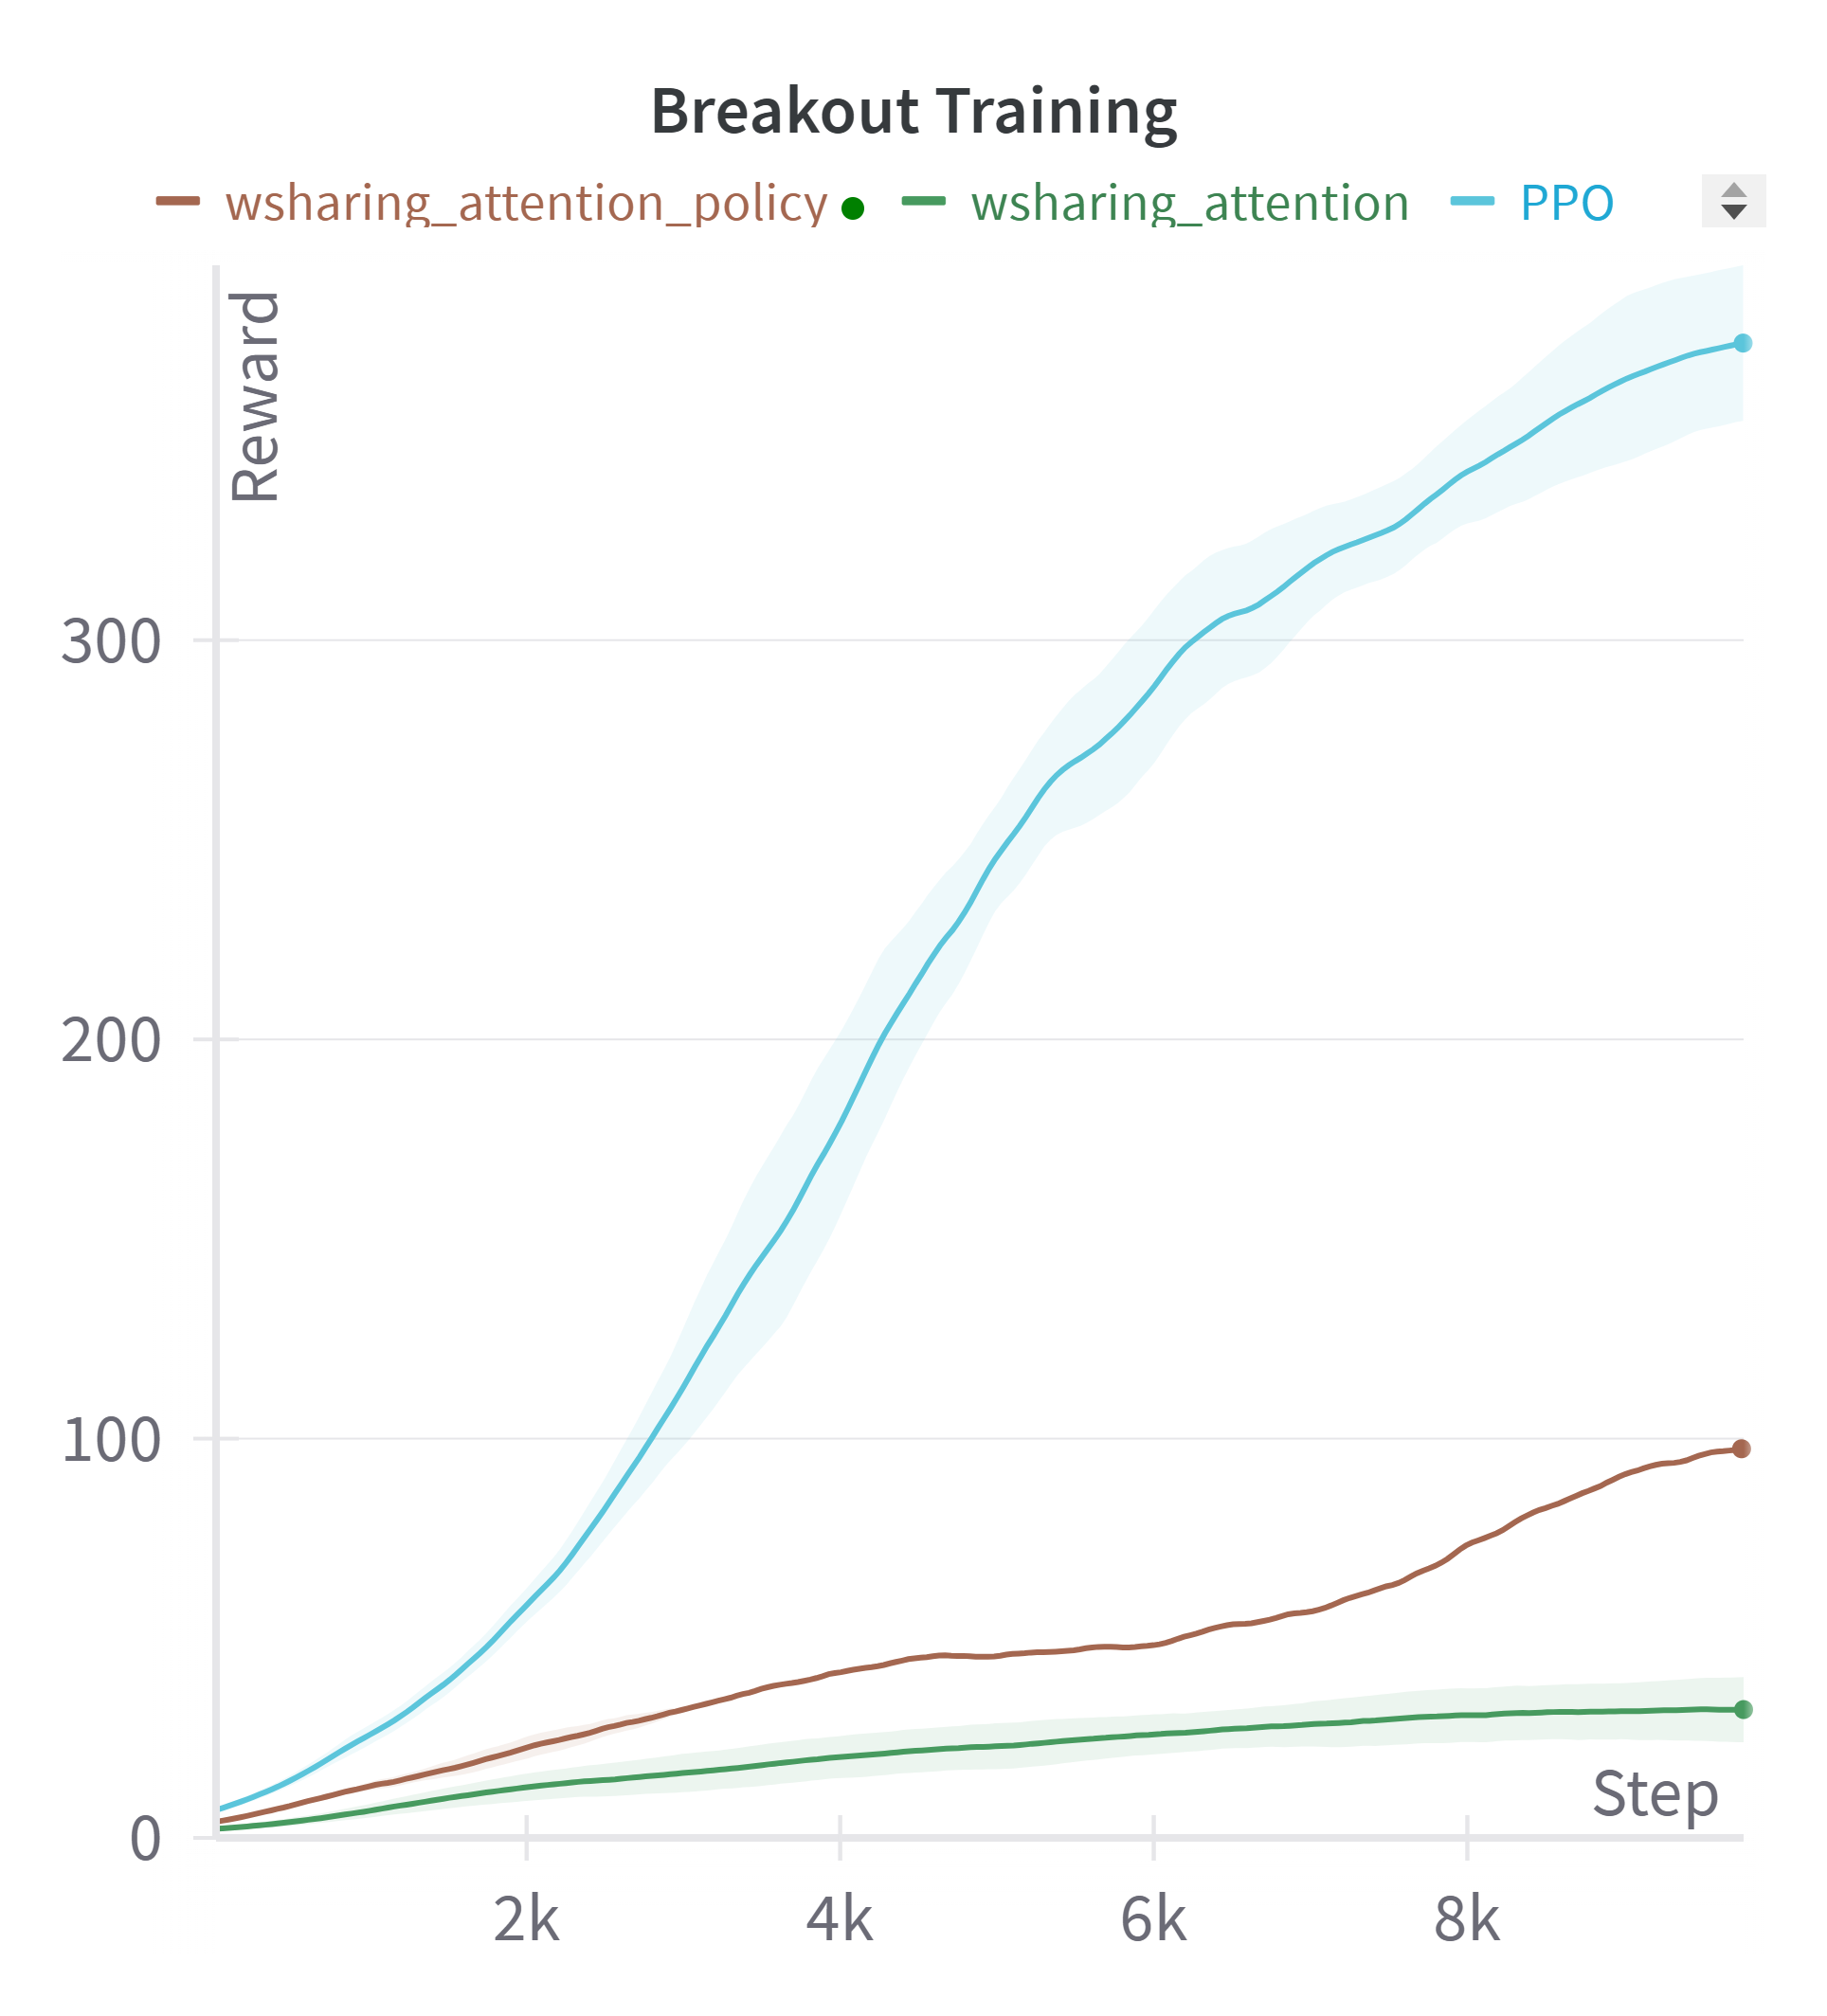
\includegraphics[width=\textwidth]{images/breakout_policy.png}
        \caption{Increasing MLP size}
        \label{fig:breakout_policy}
    \end{subfigure}
    \hfill
    \begin{subfigure}[b]{0.32\textwidth}
        \centering
        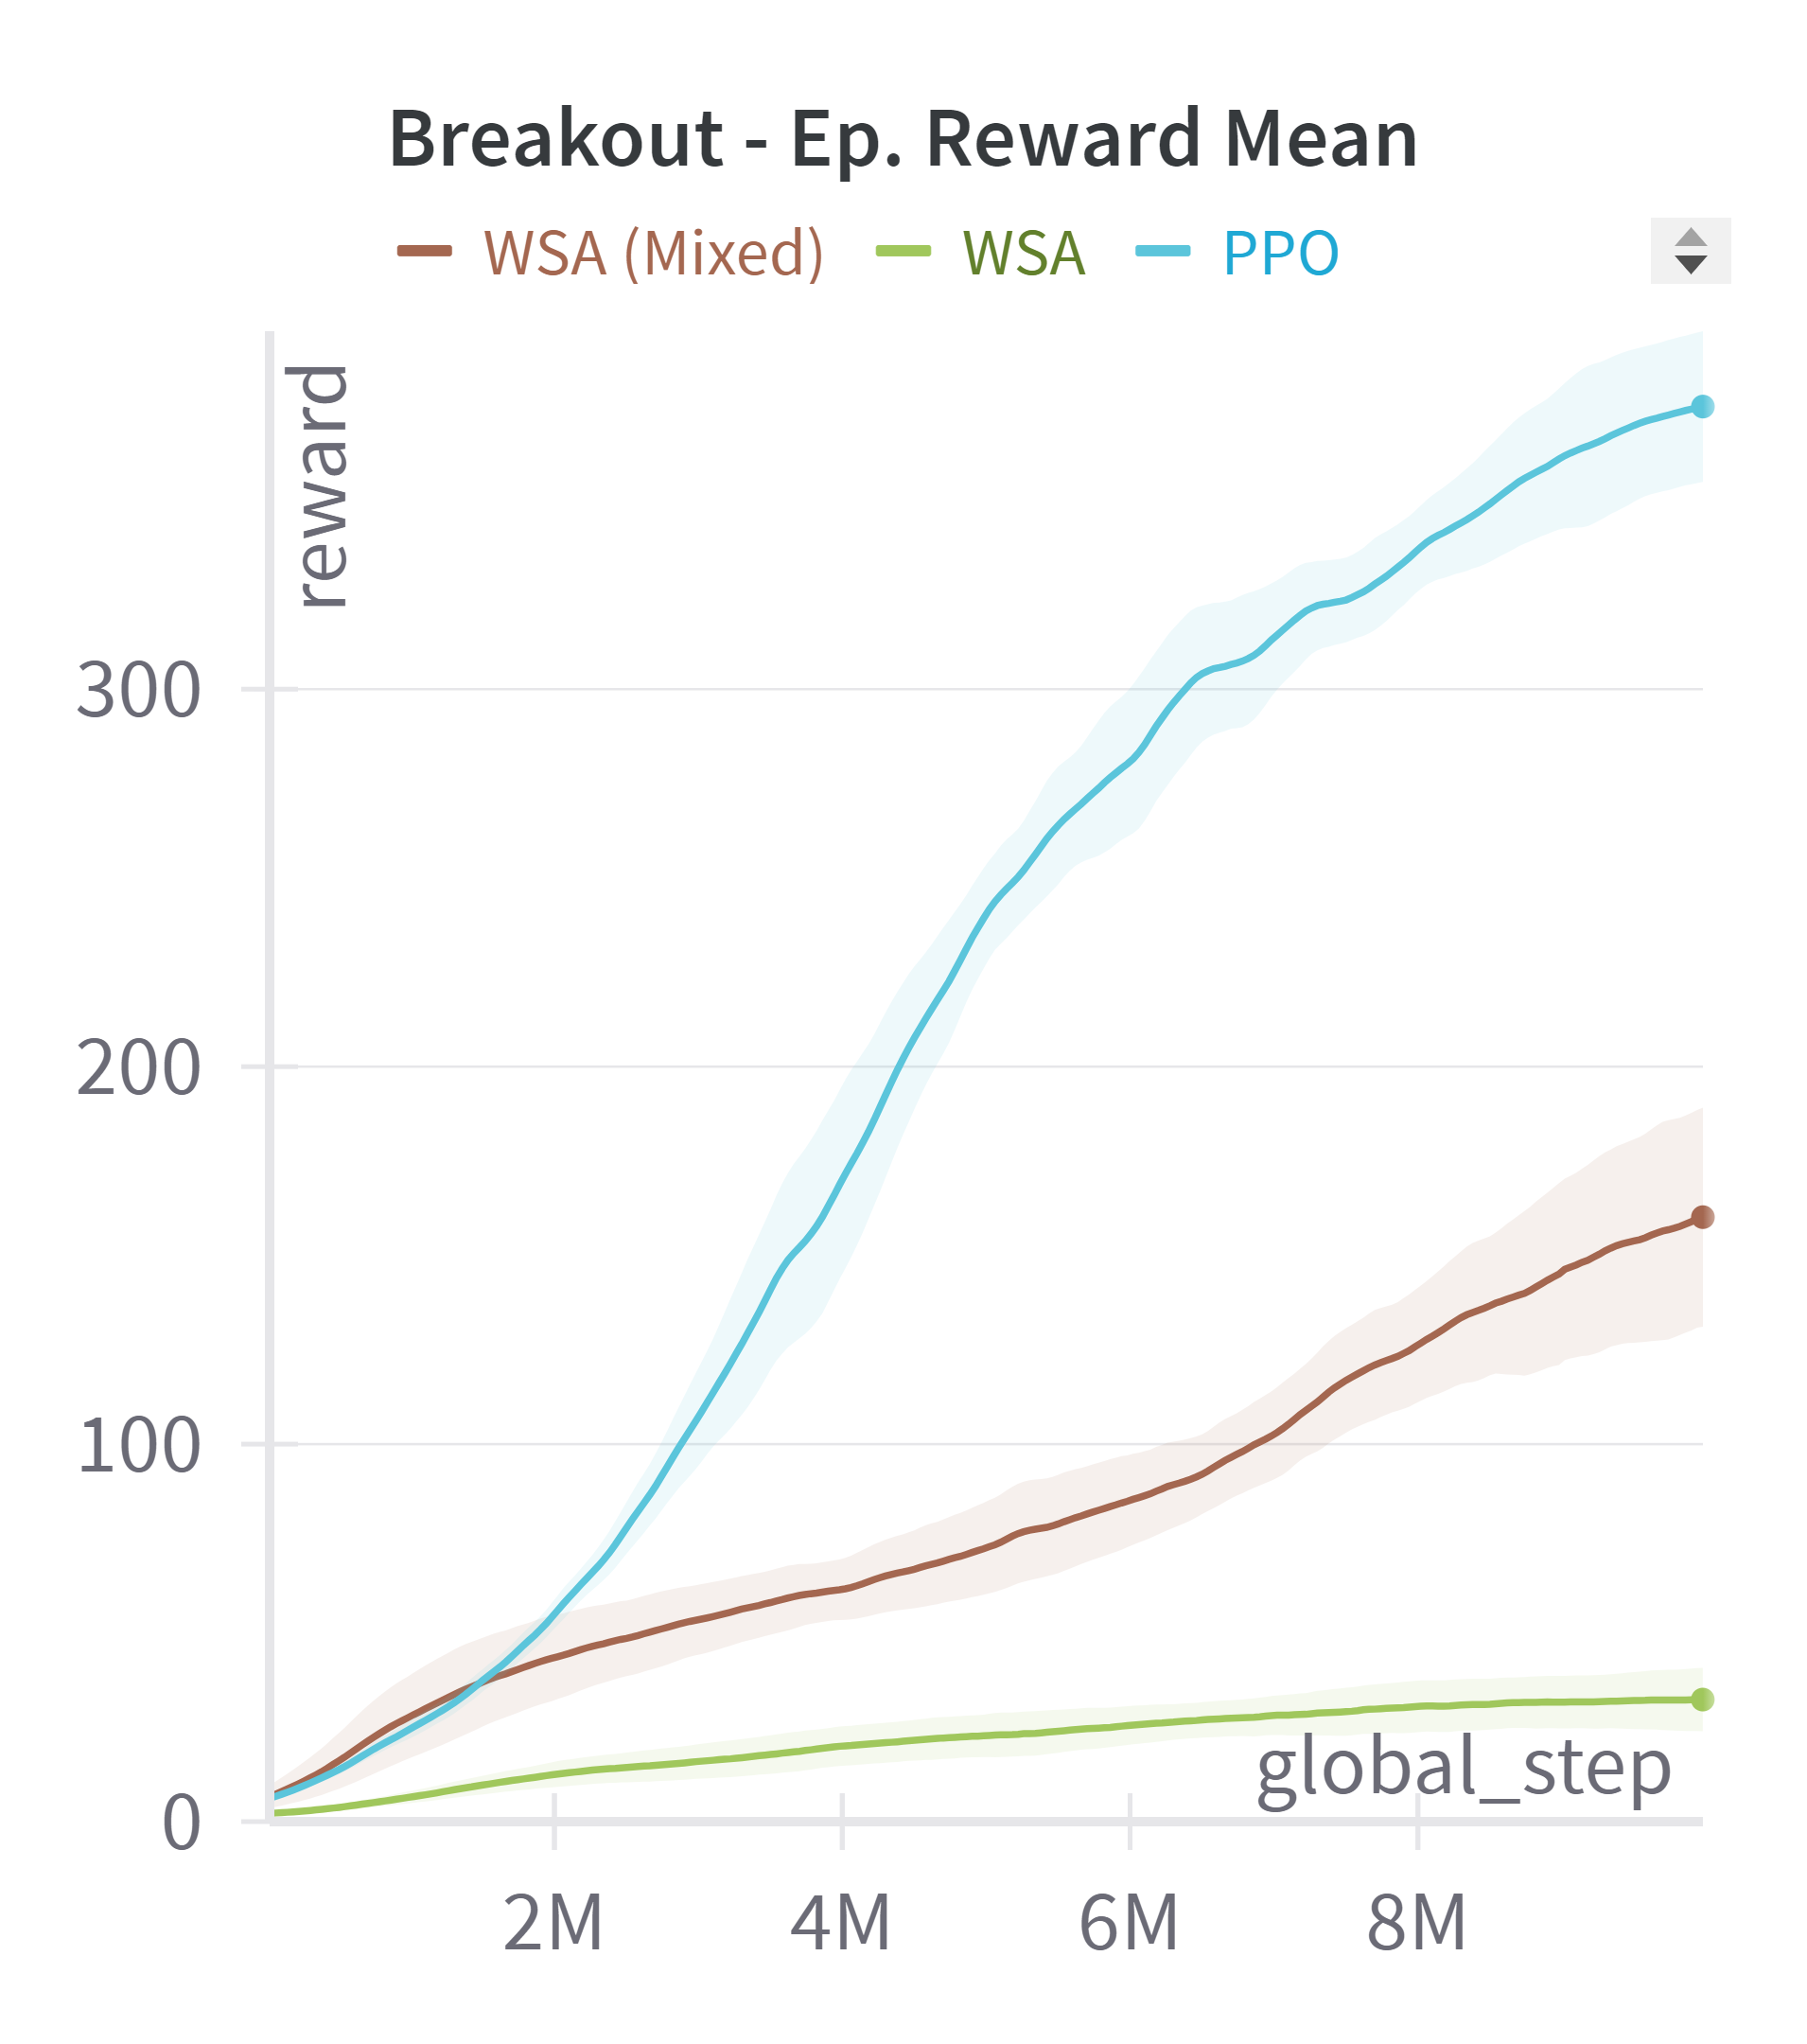
\includegraphics[width=\textwidth]{images/breakout_expert.png}
        \caption{Using Mixed Data}
        \label{fig:breakout_expert}
    \end{subfigure}
    \hfill
    \begin{subfigure}[b]{0.32\textwidth}
        \centering
        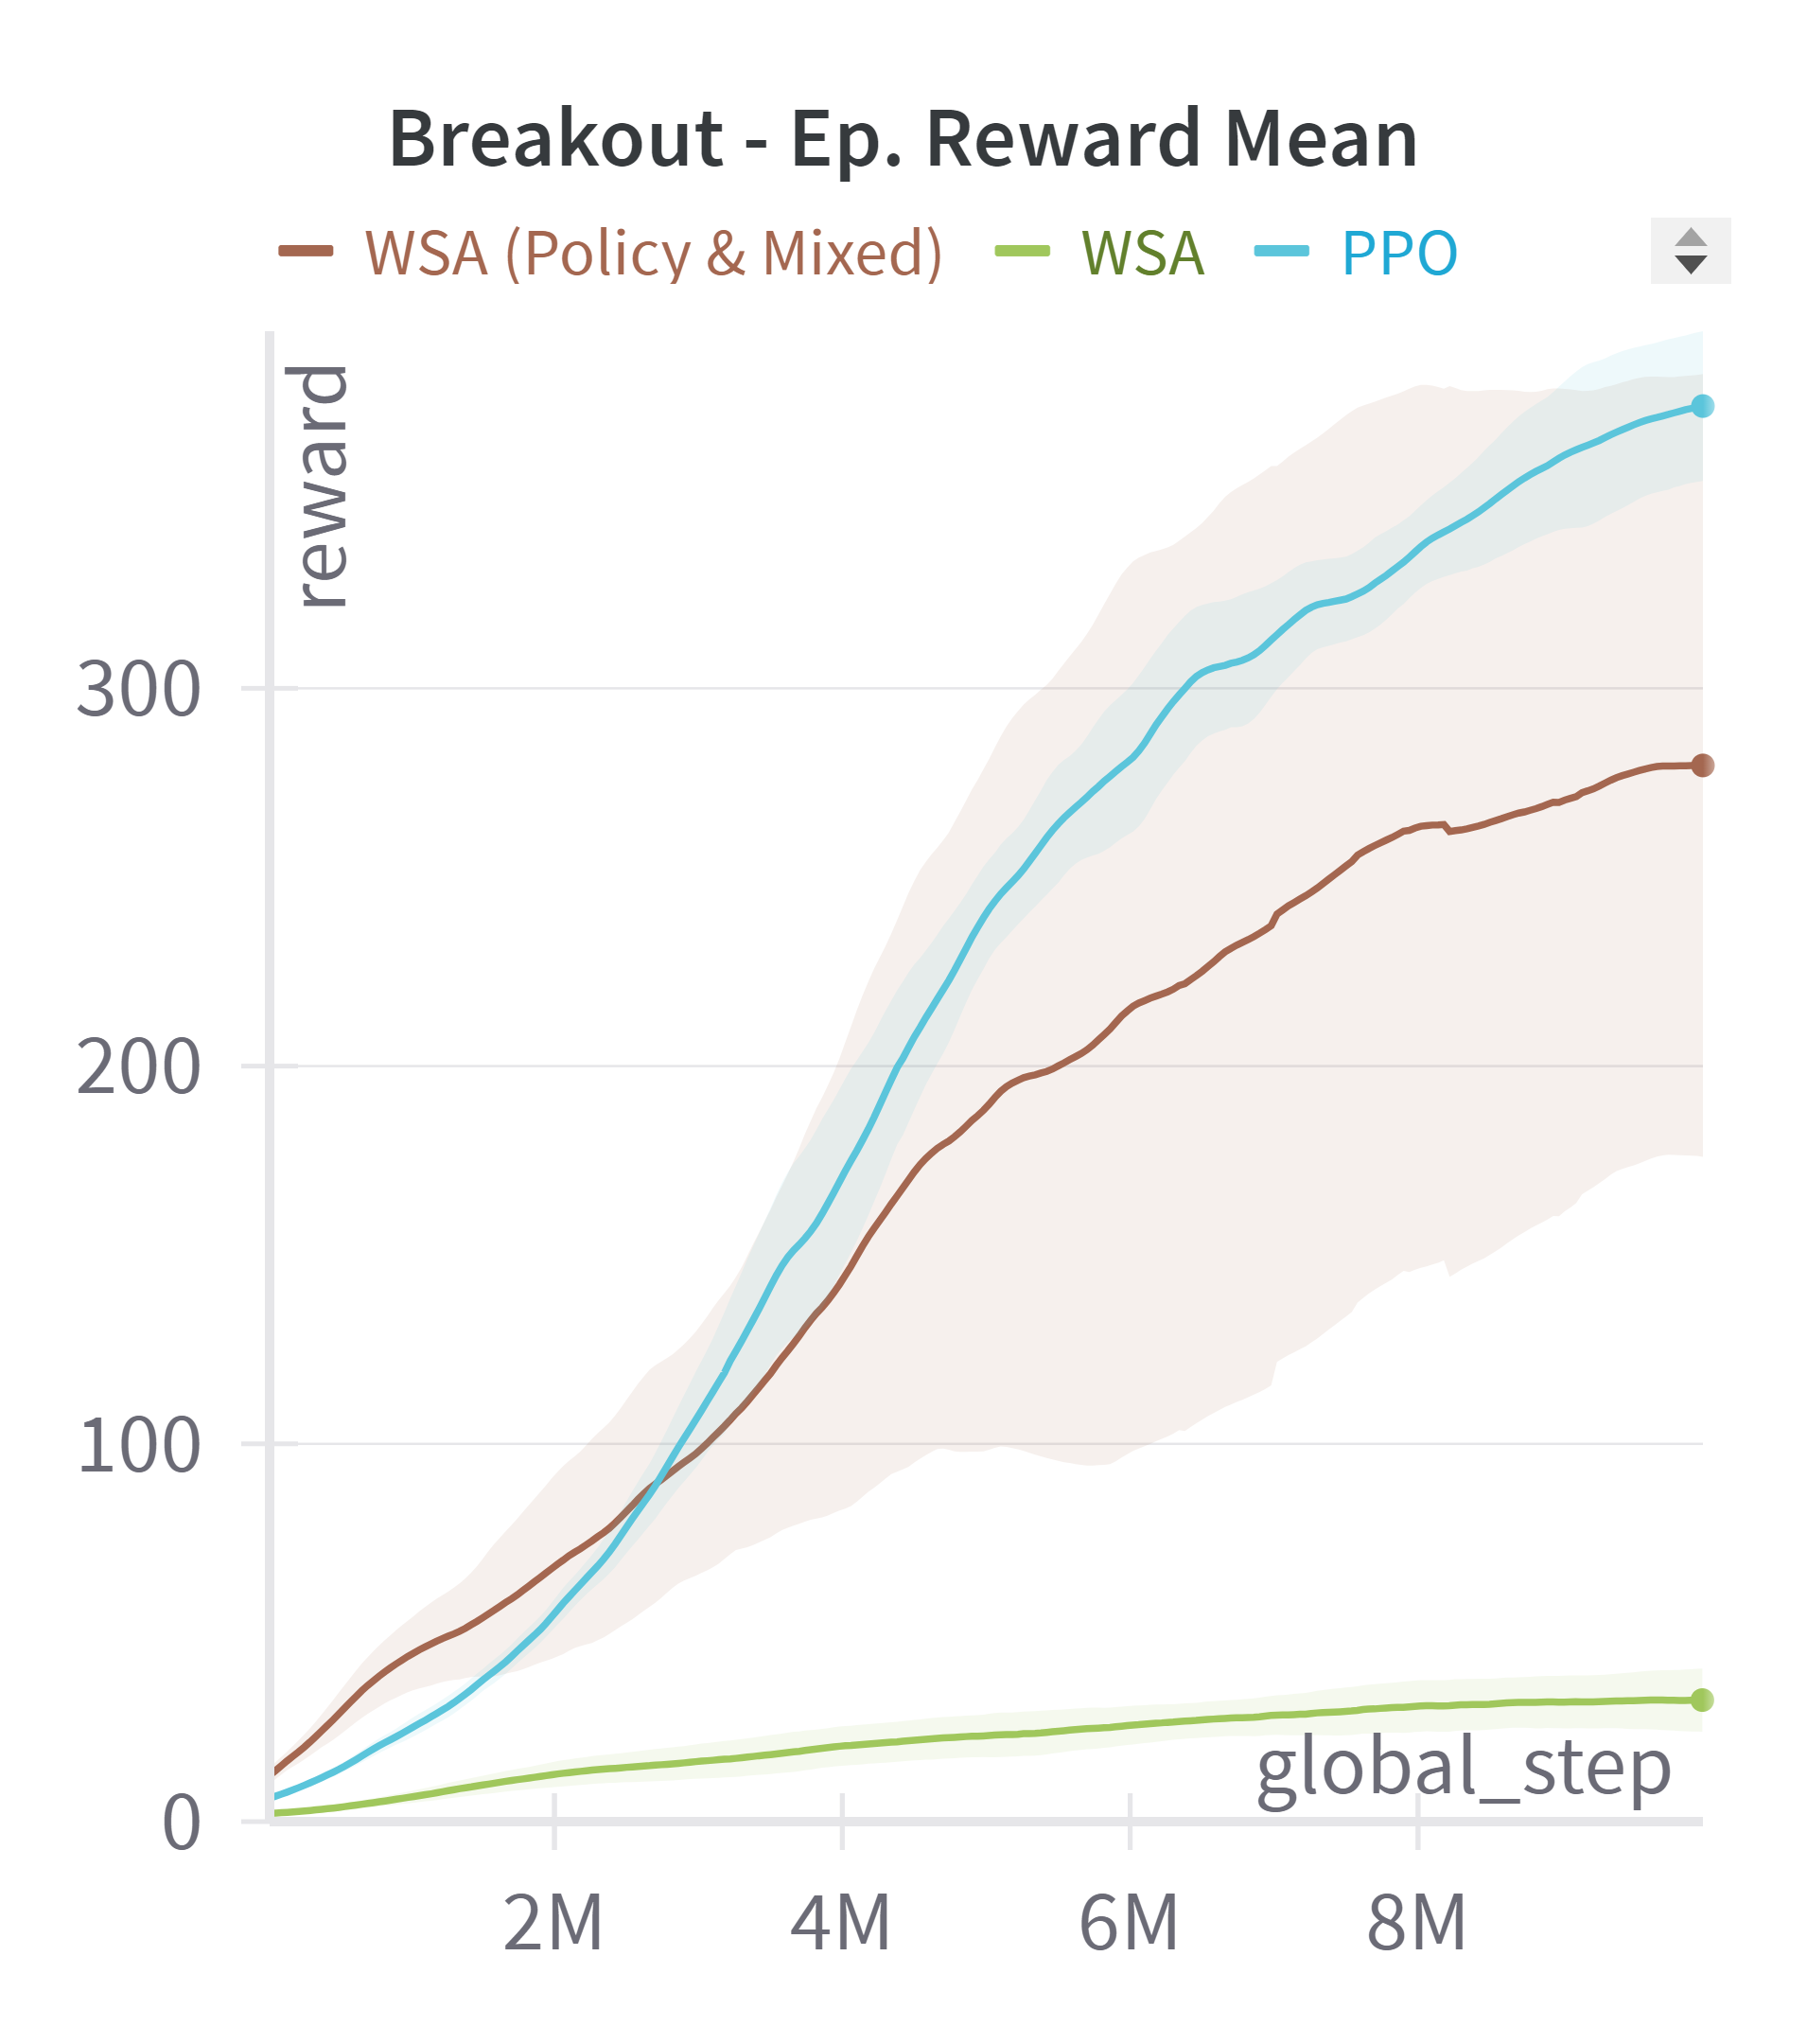
\includegraphics[width=\textwidth]{images/breakout_policy_mixed.png}
        \caption{Mixed Data + Increased MLP}
        \label{fig:breakout_expert_policy}
    \end{subfigure}
    \caption{Performance comparison of WSA with PPO across various strategies on \texttt{Breakout}. Each subfigure displays the average score with the standard deviation shaded. They report the different experiments to improve the performance of WSA: (\ref{fig:breakout_policy}) increasing the size of the \texttt{Fully-Connected Network} on performance, (\ref{fig:breakout_expert}) pre-training the models using random data and expert data, and (\ref{fig:breakout_expert_policy}) combining the effect of increased \texttt{Fully-Connected Network} and expert data during pre-training.}
    \label{fig:breakout_study}
\end{figure}


\begin{table}[ht]
\centering
    \begin{tabular}[b]{lll}
                \multicolumn{1}{l}{Environment}  &\multicolumn{1}{l}{\bf Agent} &\multicolumn{1}{l}{\bf Reward} \\
                \hline \\


                \multirow{3}{*}{\texttt{Breakout}}
                                      & CNN & 65.98 $\pm$ 1.62 \\
                                      & FIX & 87.17 $\pm$ 6.87 \\
                                      & WSA & 99.58 $\pm$ 6.66 \\

                \multirow{3}{*}{\texttt{Breakout - Policy}}
                                      & CNN & 118.71 $\pm$ 4.30 \\
                                      & FIX & 106.46 $\pm$ 10.84 \\
                                      & WSA & 156.17 $\pm$ 3.59 \\

                \multirow{3}{*}{\texttt{Breakout - Mixed}}
                                      & CNN & 62.21 $\pm$ 1.98 \\
                                      & \underline{FIX} & \underline{199.08 $\pm$ 7.46}\\
                                      & WSA & 345.52 $\pm$ 6.47 \\

                \multirow{4}{*}{\texttt{Breakout - Policy \& Mixed}}
                                      & CNN & 68.51 $\pm$ 1.85 \\
                                      & FIX & 71.06 $\pm$ 5.04 \\
                                      & \underline{WSA} & \underline{387.15 $\pm$ 0.43} \\ \\


                                      & \textbf{PPO} & \textbf{413.51 $\pm$ 1.10}\\
    \end{tabular}
    \caption{TODO}
    \label{tab:breakout_results}
\end{table}




\section{Weight Sharing Attention Explainability}\label{sec:explainability}
TODO
%Lastly, Figure \ref{fig:inter} illustrates the enhanced \texttt{explainability} provided by WSA. By examining the current frames and the corresponding weights allocated by the shared component to each pre-trained model, one can appreciate agents' decision-making process. The visualization reveals how various FMs are leveraged in distinct contexts, shedding light on agents' dynamic adaptation of its prior knowledge.

\section{DQN}
TODO










%
%
%% mio vecchio
%As can be seen from the graphs of the learning curves, in some cases such as Pong and Ms. Pacman, the various skilled agents manage to learn faster than standard PPO. Meanwhile, in Asteroids, the learning speed is comparable with PPO.
%The chosen skills track moving objects and are very useful in games such as Pong whose underlying environment does not change as the game progresses, this allows the agent to learn faster by concentrating only on the moving ball and moving bars instead of the whole game frame.
%
%%analisi su breakout
%Regarding Breakout, an initial analysis of the experiments performed shows that skill-equipped agents are not competitive with a PPO agent. This could be for various reasons, such as the fact that the skills are only trained on frames where the agent plays randomly, and as Breakout is a game where the structure changes as it progresses when the bricks are destroyed, the skills may no longer be informative in the middle or final stages of the game and even confuse the agent.
%Another reason could be the fact that the skills used so far mostly track moving objects, which in Breakout are the ball and the bar. The agent may therefore have little or no information about the bricks, which are a static part of the frame.
%One more reason could be that the policy learning part of the algorithm was untouched and bigger networks may extract more information from the skills.
%
%To this end, we have made other experiments by first collecting a dataset of 1000 episodes, 500 of which are frames of an agent that plays random while the other 500 are collected using a trained PPO agent. In this way, we added variety to the dataset and we trained again the skills using this new data. We refer to these skills as \textbf{expert skills}.
%As extractors, we restricted the tests only to the use of Weights Sharing with sizes 1024 and 256, as these are the ones that performed best in the other experiments, we then chose for comparison Reservoir extractor with size 1024 and Combine. We also decided to focus only on a subset of extractors to decrease the testing time.
%The results of this experiment can be seen in Fig. \ref{fig:breakout_expert}
%
%Next, we ran another experiment using expert skills and also increasing the policy network dimension of the algorithm. Standard PPO uses a linear layer of size 256 both for the policy network and value function network, we instead increased this network using three linear layers of size 1024, 512, and 256 respectively for the first, second, and third one. We use ReLU as activation function after each linear layer to add non-linearity.
%The results are shown in Fig \ref{fig:breakout_expert_and_policy}.
%
%Finally, the last round of experiments was conducted by including the skills of Image Completion and Frame Prediction in addition to the three previously used. The skills are all used in expert mode and we also increased the policy learning network as before.
%For this last experiment, we used only the agent that performed best in the other experiments, namely Weights sharing with embedding dimensions 256 and 1024.
%Fig. \ref{fig:breakout_expert_policy_skills} shows the results.
%
%\begin{figure}[htbp]
%    \centering
%    \begin{subfigure}[b]{0.32\textwidth}
%        \centering
%        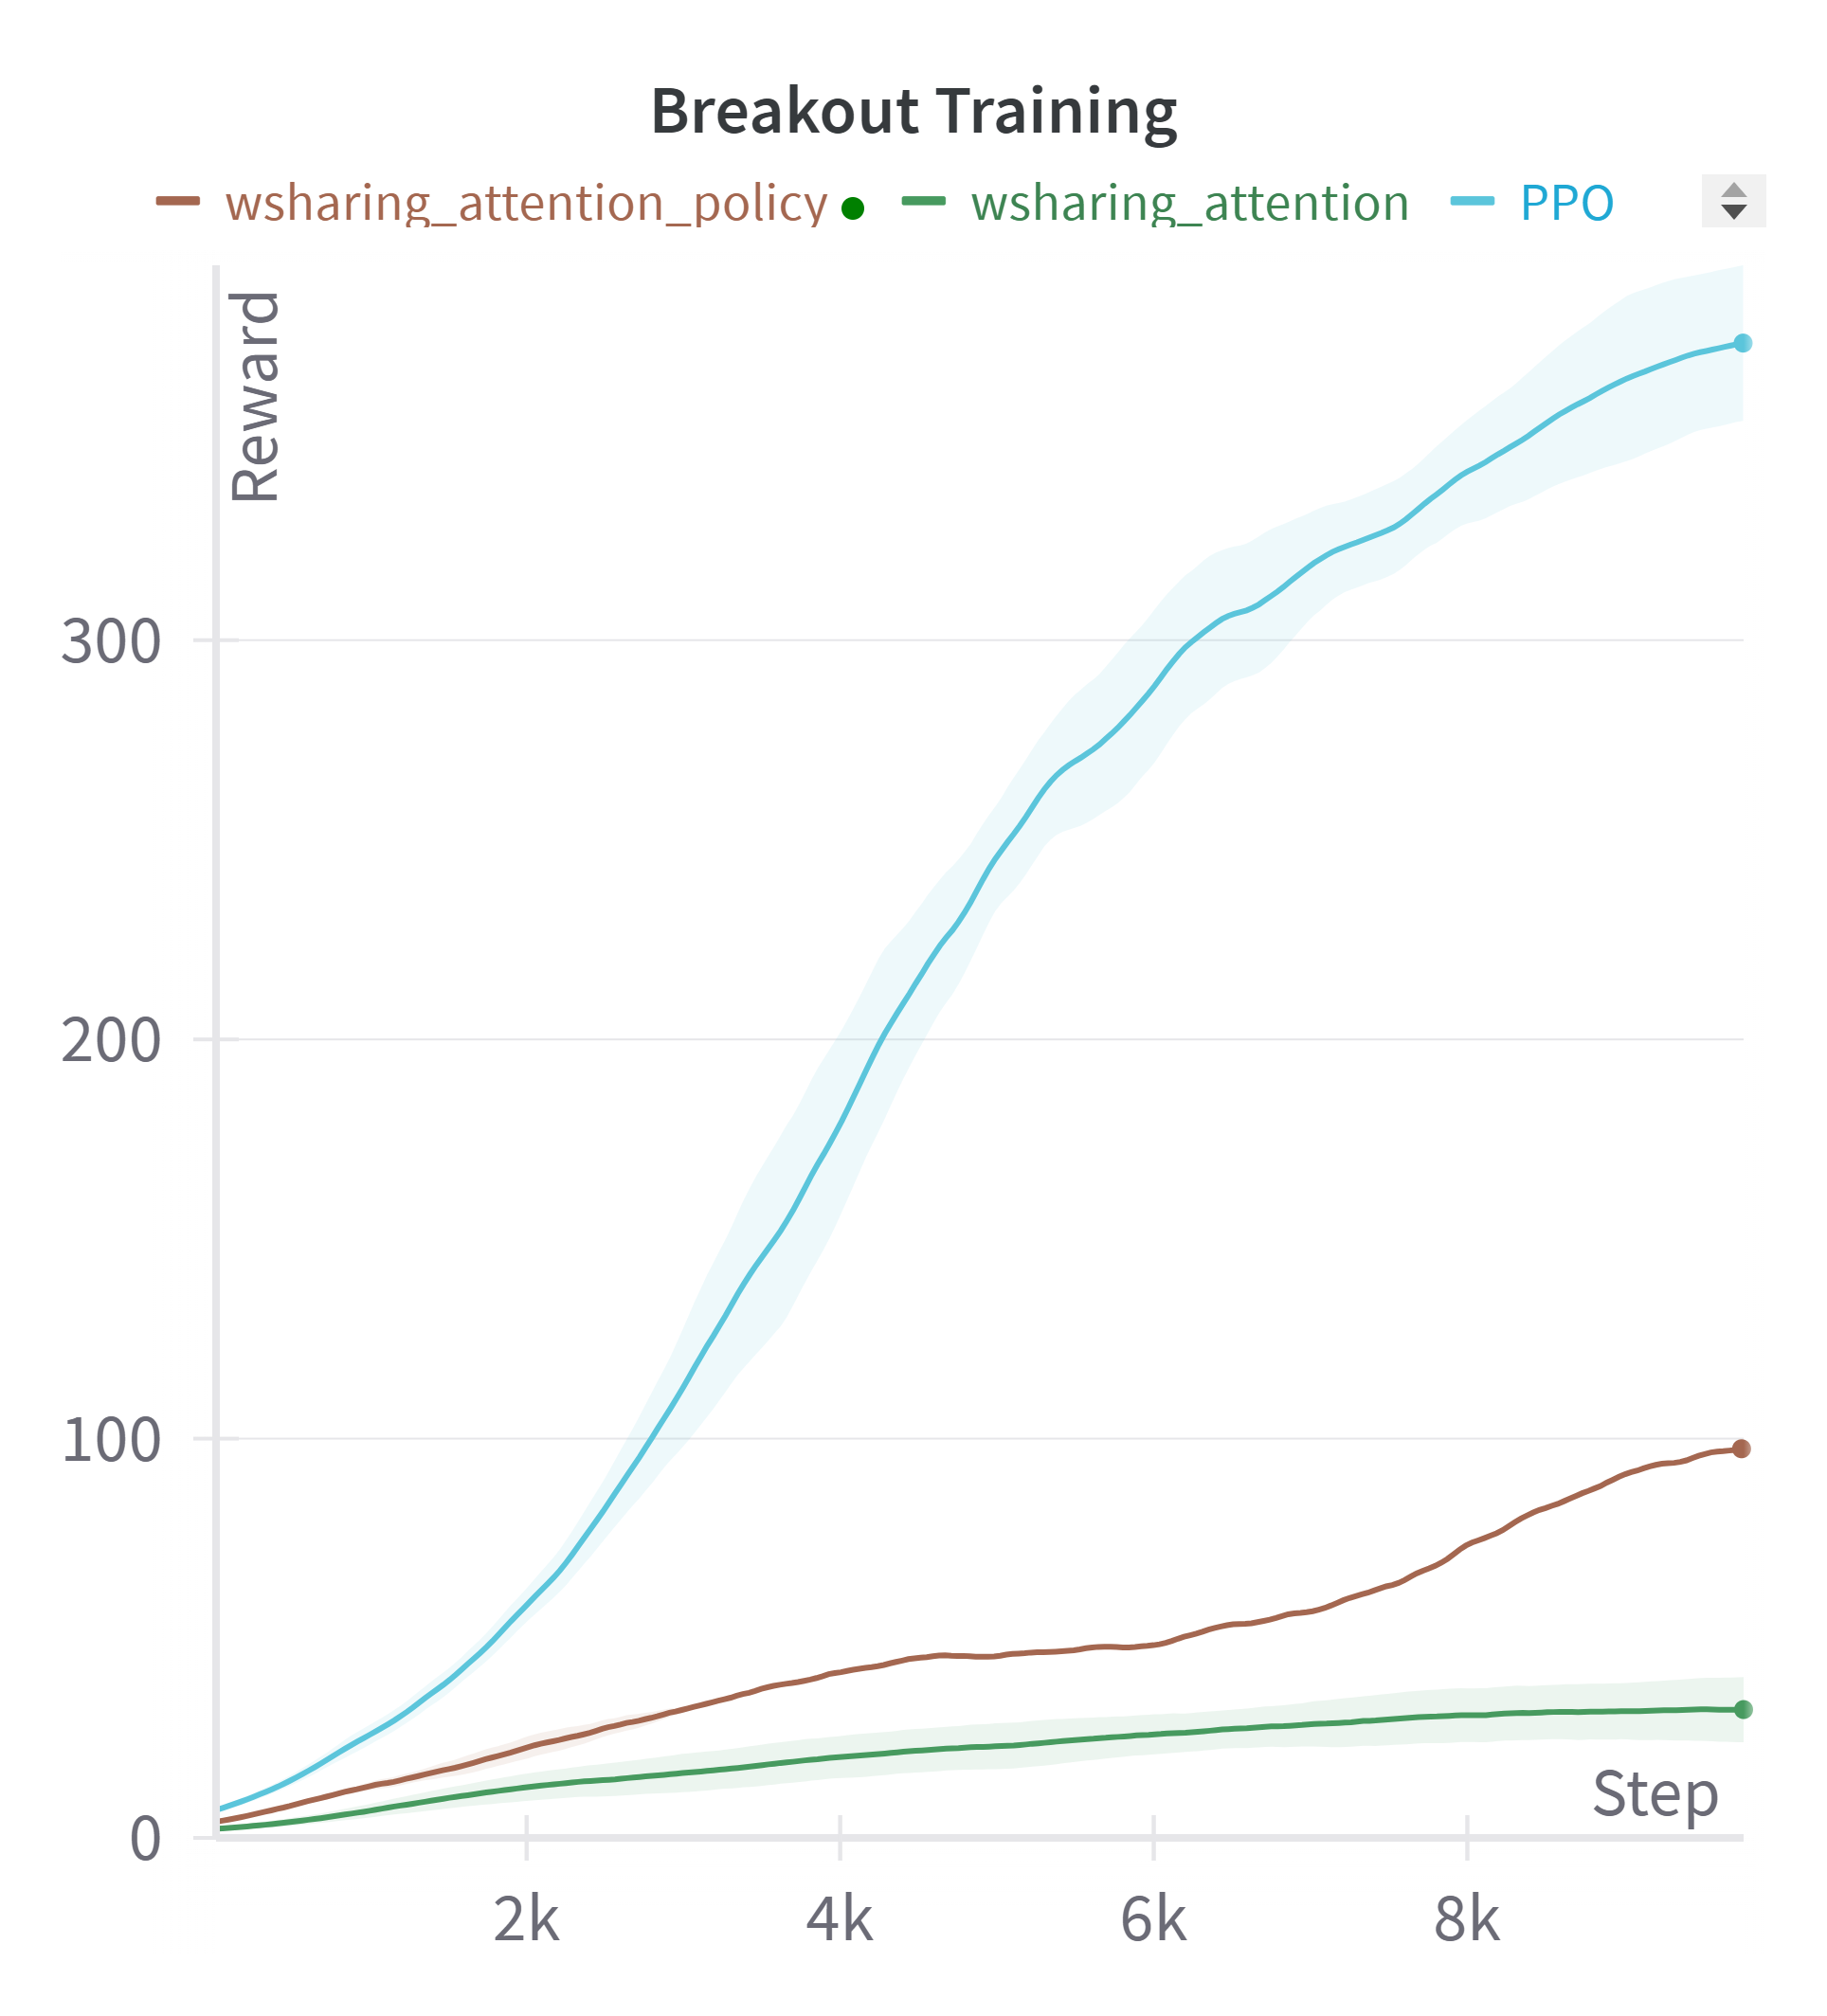
\includegraphics[width=\textwidth]{images/breakout_policy.png}
%        \caption{Breakout con MLP + quello che faceva schifo}
%        \label{fig:breakout_expert}
%    \end{subfigure}
%    \hfill
%    \begin{subfigure}[b]{0.32\textwidth}
%        \centering
%        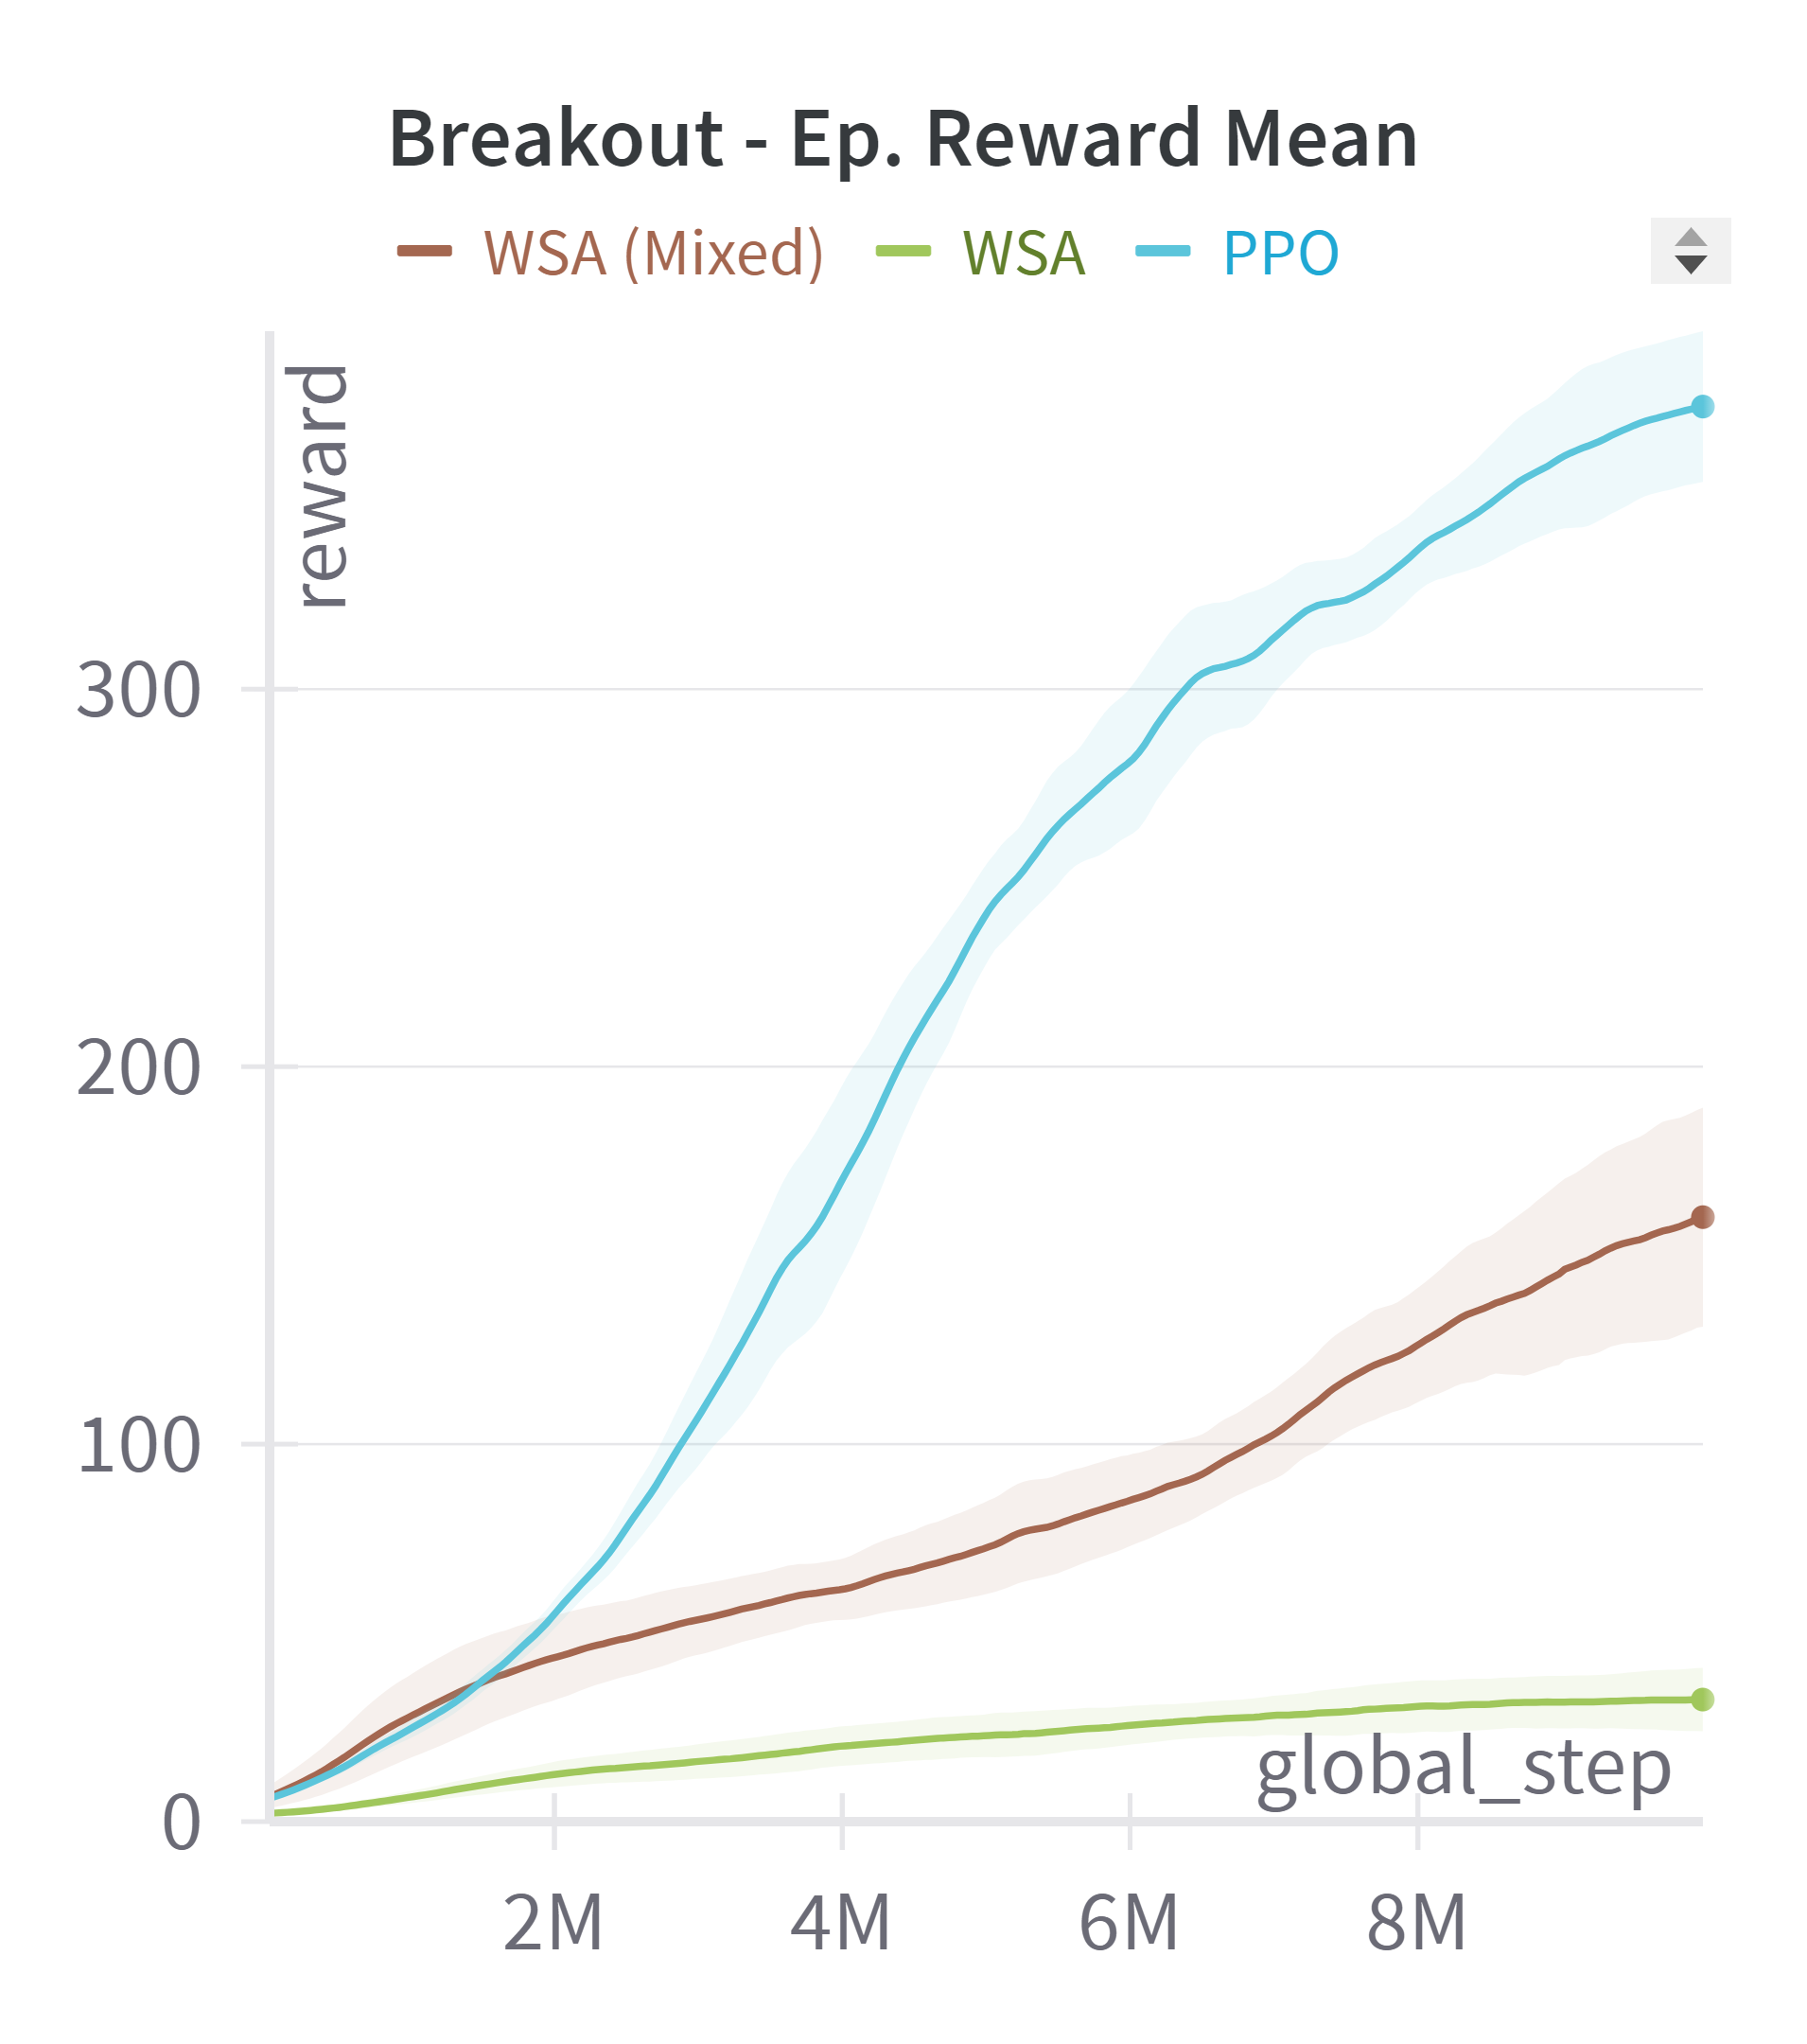
\includegraphics[width=\textwidth]{images/breakout_expert.png}
%        \caption{Breakout stesso di prima ma con dati expert}
%        \label{fig:breakout_expert_and_policy}
%    \end{subfigure}
%    \hfill
%    \begin{subfigure}[b]{0.32\textwidth}
%        \centering
%        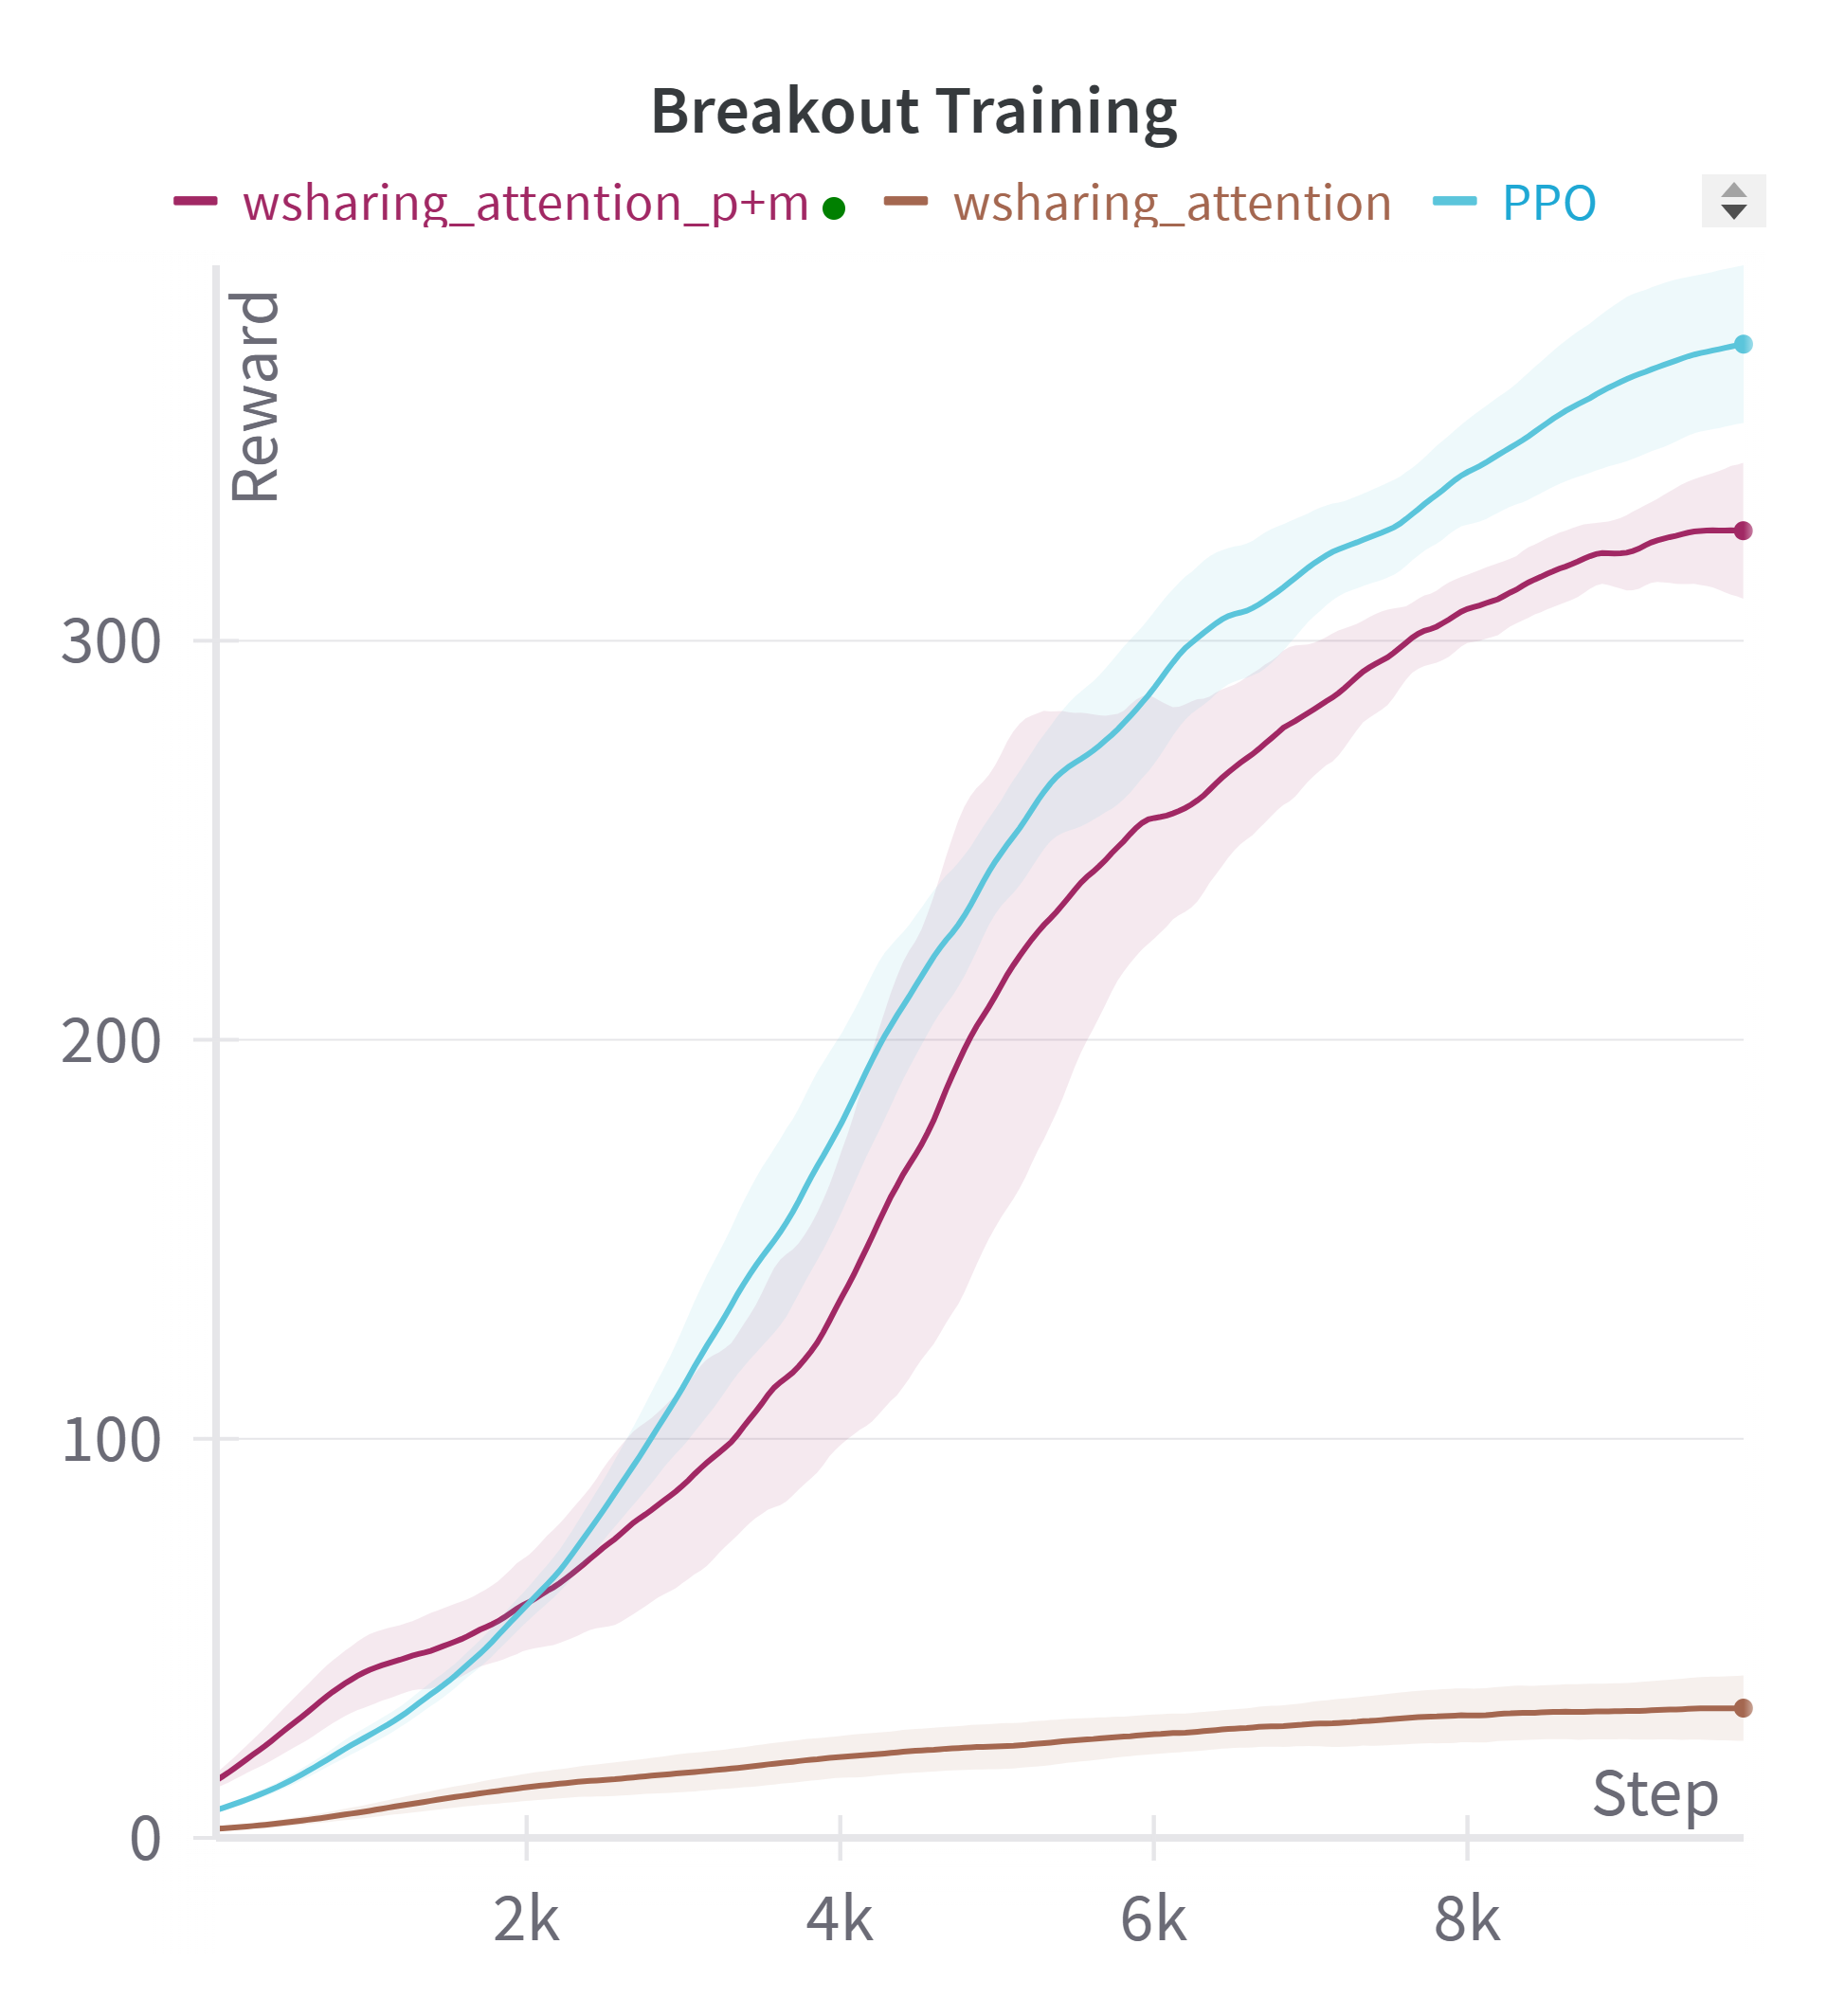
\includegraphics[width=\textwidth]{images/breakout_p+m.png}
%        \caption{Breakout expert  + policy}
%        \label{fig:breakout_expert_policy_skills}
%    \end{subfigure}
%    \hfill
%
%    \caption{PPO
% rimane uguale in tutti e 3}
%    \label{fig:trainresults}
%\end{figure}
%
%
%
%Tab. \ref{tab:results} shows the highest reward obtained for each game by the top three agents of each game considering the evaluation. This table also presents the agent called PPO which represents our training run of a standard PPO agent without skills, and the agent REFERENCE which is the result reported on the Hugging Face page of Stable-Baselines.
%
%\begin{table}[htbp]
%    \begin{center}
%        \begin{tabular}{llll}
%            \multicolumn{1}{l}{AGENT}  &\multicolumn{1}{l}{\bf PONG} &\multicolumn{1}{l}{\bf BREAKOUT} &\multicolumn{1}{l}{\bf MS. PACMAN}
%            \\ \hline \\
%            Weights Sharing (1024) &  20 $\pm$ 00 &  - &  -  \\
%            Weights Sharing (256)  &  - &  356 $\pm$ 00 &  2487 $\pm$ 00  \\
%            Reservoir (1024)       &  20 $\pm$ 00 &  - &  2111 $\pm$ 00 \\
%            CNN (2)                &  20 $\pm$ 00 &  - &  1812 $\pm$ 00 \\
%            CNN (3)                &  - &  50 $\pm$ 00 &  - \\
%            Fixed Lin. (512)                &  - &  50 $\pm$ 00 &  - \\
%            PPO                    &  20 $\pm$ 00 &  387 $\pm$ 00 &  2230 $\pm$ 00 \\
%            REFERENCE              &  21 $\pm$ 0 &  398 $\pm$ 16.30 &  1659 $\pm$ 144.81 \\
%        \end{tabular}
%    \end{center}
%    \caption{Tra parentesi le dimensioni}
%    \label{tab:results}
%\end{table}

%As can be seen in \ref{fig:breakout_expert} we tested Breakout with expert skills only on a subset of a few extractors. We chose Weights Sharing Attention with 256 and 1024 as dimensions for skills embeddings, Combine Extractor, and Reservoir Extractor with 1024 as dimension of the reservoir. We restricted only to these extractors to increase the time for experiments too much.
%We can see that only by using expert skills the Weights Sharing agent become comparable with the PPO agent, it learns more slowly but eventually in evaluation manages to have a score very similar to PPO. Reaching xxx while PPO reaches xxx.

%Let us now analyze the use of expert skills and the increase of the network involved in policy learning.
%We can see in Fig. \ref{fig:breakout_expert_and_policy} that Weights Sharing Attention with dimension 256 for skills embeddings is the one that performs the best. It is comparable with a PPO agent since they perform basically the same.



%analisi weights sharing
%In most of the experiments we have performed, we have noticed that weights sharing attention as a way of concatenating different skill embeddings is the one that performs best.
%It, being more general as a method manages to better filter out noisy input, focusing only on the information that is really important for the agent to learn.

%INSERIRE ANALISI SUL NUMERO DI PARAMETRI TOTALI DI PPO E SKILLED AGENT

%INSERIRE ANALISI SUGLI FPS TRA PPO E SKILLED AGENT
